% Options for packages loaded elsewhere
% Options for packages loaded elsewhere
\PassOptionsToPackage{unicode}{hyperref}
\PassOptionsToPackage{hyphens}{url}
\PassOptionsToPackage{dvipsnames,svgnames,x11names}{xcolor}
%
\documentclass[
  english,
  11pt,
  letterpaper,
]{scrbook}
\usepackage{xcolor}
\usepackage[paperwidth=6in,paperheight=9in,inner=0.75in,outer=0.5in,top=0.6in,bottom=0.75in,heightrounded]{geometry}
\usepackage{amsmath,amssymb}
\setcounter{secnumdepth}{5}
\usepackage{iftex}
\ifPDFTeX
  \usepackage[T1]{fontenc}
  \usepackage[utf8]{inputenc}
  \usepackage{textcomp} % provide euro and other symbols
\else % if luatex or xetex
  \usepackage{unicode-math} % this also loads fontspec
  \defaultfontfeatures{Scale=MatchLowercase}
  \defaultfontfeatures[\rmfamily]{Ligatures=TeX,Scale=1}
\fi
\usepackage{lmodern}
\ifPDFTeX\else
  % xetex/luatex font selection
\fi
% Use upquote if available, for straight quotes in verbatim environments
\IfFileExists{upquote.sty}{\usepackage{upquote}}{}
\IfFileExists{microtype.sty}{% use microtype if available
  \usepackage[]{microtype}
  \UseMicrotypeSet[protrusion]{basicmath} % disable protrusion for tt fonts
}{}
\makeatletter
\@ifundefined{KOMAClassName}{% if non-KOMA class
  \IfFileExists{parskip.sty}{%
    \usepackage{parskip}
  }{% else
    \setlength{\parindent}{0pt}
    \setlength{\parskip}{6pt plus 2pt minus 1pt}}
}{% if KOMA class
  \KOMAoptions{parskip=half}}
\makeatother
% Make \paragraph and \subparagraph free-standing
\makeatletter
\ifx\paragraph\undefined\else
  \let\oldparagraph\paragraph
  \renewcommand{\paragraph}{
    \@ifstar
      \xxxParagraphStar
      \xxxParagraphNoStar
  }
  \newcommand{\xxxParagraphStar}[1]{\oldparagraph*{#1}\mbox{}}
  \newcommand{\xxxParagraphNoStar}[1]{\oldparagraph{#1}\mbox{}}
\fi
\ifx\subparagraph\undefined\else
  \let\oldsubparagraph\subparagraph
  \renewcommand{\subparagraph}{
    \@ifstar
      \xxxSubParagraphStar
      \xxxSubParagraphNoStar
  }
  \newcommand{\xxxSubParagraphStar}[1]{\oldsubparagraph*{#1}\mbox{}}
  \newcommand{\xxxSubParagraphNoStar}[1]{\oldsubparagraph{#1}\mbox{}}
\fi
\makeatother


\usepackage{longtable,booktabs,array}
\newcounter{none} % for unnumbered tables
\usepackage{calc} % for calculating minipage widths
% Correct order of tables after \paragraph or \subparagraph
\usepackage{etoolbox}
\makeatletter
\patchcmd\longtable{\par}{\if@noskipsec\mbox{}\fi\par}{}{}
\makeatother
% Allow footnotes in longtable head/foot
\IfFileExists{footnotehyper.sty}{\usepackage{footnotehyper}}{\usepackage{footnote}}
\makesavenoteenv{longtable}
\usepackage{graphicx}
\makeatletter
\newsavebox\pandoc@box
\newcommand*\pandocbounded[1]{% scales image to fit in text height/width
  \sbox\pandoc@box{#1}%
  \Gscale@div\@tempa{\textheight}{\dimexpr\ht\pandoc@box+\dp\pandoc@box\relax}%
  \Gscale@div\@tempb{\linewidth}{\wd\pandoc@box}%
  \ifdim\@tempb\p@<\@tempa\p@\let\@tempa\@tempb\fi% select the smaller of both
  \ifdim\@tempa\p@<\p@\scalebox{\@tempa}{\usebox\pandoc@box}%
  \else\usebox{\pandoc@box}%
  \fi%
}
% Set default figure placement to htbp
\def\fps@figure{htbp}
\makeatother


% definitions for citeproc citations
\NewDocumentCommand\citeproctext{}{}
\NewDocumentCommand\citeproc{mm}{%
  \begingroup\def\citeproctext{#2}\cite{#1}\endgroup}
\makeatletter
 % allow citations to break across lines
 \let\@cite@ofmt\@firstofone
 % avoid brackets around text for \cite:
 \def\@biblabel#1{}
 \def\@cite#1#2{{#1\if@tempswa , #2\fi}}
\makeatother
\newlength{\cslhangindent}
\setlength{\cslhangindent}{1.5em}
\newlength{\csllabelwidth}
\setlength{\csllabelwidth}{3em}
\newenvironment{CSLReferences}[2] % #1 hanging-indent, #2 entry-spacing
 {\begin{list}{}{%
  \setlength{\itemindent}{0pt}
  \setlength{\leftmargin}{0pt}
  \setlength{\parsep}{0pt}
  % turn on hanging indent if param 1 is 1
  \ifodd #1
   \setlength{\leftmargin}{\cslhangindent}
   \setlength{\itemindent}{-1\cslhangindent}
  \fi
  % set entry spacing
  \setlength{\itemsep}{#2\baselineskip}}}
 {\end{list}}
\usepackage{calc}
\newcommand{\CSLBlock}[1]{\hfill\break\parbox[t]{\linewidth}{\strut\ignorespaces#1\strut}}
\newcommand{\CSLLeftMargin}[1]{\parbox[t]{\csllabelwidth}{\strut#1\strut}}
\newcommand{\CSLRightInline}[1]{\parbox[t]{\linewidth - \csllabelwidth}{\strut#1\strut}}
\newcommand{\CSLIndent}[1]{\hspace{\cslhangindent}#1}

\ifLuaTeX
\usepackage[bidi=basic,shorthands=off]{babel}
\else
\usepackage[bidi=default,shorthands=off]{babel}
\fi
\ifLuaTeX
  \usepackage{selnolig} % disable illegal ligatures
\fi


\setlength{\emergencystretch}{3em} % prevent overfull lines

\providecommand{\tightlist}{%
  \setlength{\itemsep}{0pt}\setlength{\parskip}{0pt}}



 


% Index support: \index{...} entries in chapters land here.
% Quarto's PDF engine loop runs makeindex automatically when .idx appears.
\usepackage{imakeidx}
\makeindex[intoc=true]
\makeatletter
\@ifpackageloaded{tcolorbox}{}{\usepackage[skins,breakable]{tcolorbox}}
\@ifpackageloaded{fontawesome5}{}{\usepackage{fontawesome5}}
\definecolor{quarto-callout-color}{HTML}{909090}
\definecolor{quarto-callout-note-color}{HTML}{0758E5}
\definecolor{quarto-callout-important-color}{HTML}{CC1914}
\definecolor{quarto-callout-warning-color}{HTML}{EB9113}
\definecolor{quarto-callout-tip-color}{HTML}{00A047}
\definecolor{quarto-callout-caution-color}{HTML}{FC5300}
\definecolor{quarto-callout-color-frame}{HTML}{acacac}
\definecolor{quarto-callout-note-color-frame}{HTML}{4582ec}
\definecolor{quarto-callout-important-color-frame}{HTML}{d9534f}
\definecolor{quarto-callout-warning-color-frame}{HTML}{f0ad4e}
\definecolor{quarto-callout-tip-color-frame}{HTML}{02b875}
\definecolor{quarto-callout-caution-color-frame}{HTML}{fd7e14}
\makeatother
\makeatletter
\@ifpackageloaded{bookmark}{}{\usepackage{bookmark}}
\makeatother
\makeatletter
\@ifpackageloaded{caption}{}{\usepackage{caption}}
\AtBeginDocument{%
\ifdefined\contentsname
  \renewcommand*\contentsname{Table of contents}
\else
  \newcommand\contentsname{Table of contents}
\fi
\ifdefined\listfigurename
  \renewcommand*\listfigurename{List of Figures}
\else
  \newcommand\listfigurename{List of Figures}
\fi
\ifdefined\listtablename
  \renewcommand*\listtablename{List of Tables}
\else
  \newcommand\listtablename{List of Tables}
\fi
\ifdefined\figurename
  \renewcommand*\figurename{Figure}
\else
  \newcommand\figurename{Figure}
\fi
\ifdefined\tablename
  \renewcommand*\tablename{Table}
\else
  \newcommand\tablename{Table}
\fi
}
\@ifpackageloaded{float}{}{\usepackage{float}}
\floatstyle{ruled}
\@ifundefined{c@chapter}{\newfloat{codelisting}{h}{lop}}{\newfloat{codelisting}{h}{lop}[chapter]}
\floatname{codelisting}{Listing}
\newcommand*\listoflistings{\listof{codelisting}{List of Listings}}
\makeatother
\makeatletter
\makeatother
\makeatletter
\@ifpackageloaded{caption}{}{\usepackage{caption}}
\@ifpackageloaded{subcaption}{}{\usepackage{subcaption}}
\makeatother
\usepackage{bookmark}
\IfFileExists{xurl.sty}{\usepackage{xurl}}{} % add URL line breaks if available
\urlstyle{same}
\hypersetup{
  pdftitle={The Starlight Engine},
  pdfauthor={Dr.~Rex Meridian, PhD (pending)},
  pdflang={en},
  colorlinks=true,
  linkcolor={Maroon},
  filecolor={Maroon},
  citecolor={Blue},
  urlcolor={Blue},
  pdfcreator={LaTeX via pandoc}}


\title{The Starlight Engine}
\usepackage{etoolbox}
\makeatletter
\providecommand{\subtitle}[1]{% add subtitle to \maketitle
  \apptocmd{\@title}{\par {\large #1 \par}}{}{}
}
\makeatother
\subtitle{How the Ancients Wired the Earth}
\author{Dr.~Rex Meridian, PhD (pending)}
\date{2026-07-02}
\begin{document}
\frontmatter
\maketitle

\renewcommand*\contentsname{Table of contents}
{
\setcounter{tocdepth}{2}
\tableofcontents
}

\mainmatter
\bookmarksetup{startatroot}

\chapter*{Preface: How I Found the
Signal}\label{preface-how-i-found-the-signal}
\addcontentsline{toc}{chapter}{Preface: How I Found the Signal}

\markboth{Preface: How I Found the Signal}{Preface: How I Found the
Signal}

\begin{tcolorbox}[enhanced jigsaw, arc=.35mm, bottomrule=.15mm, bottomtitle=1mm, breakable, colback=white, colbacktitle=quarto-callout-important-color!10!white, colframe=quarto-callout-important-color-frame, coltitle=black, left=2mm, leftrule=.75mm, opacityback=0, opacitybacktitle=0.6, rightrule=.15mm, title=\textcolor{quarto-callout-important-color}{\faExclamation}\hspace{0.5em}{Read this first (the publisher made me put this here)}, titlerule=0mm, toprule=.15mm, toptitle=1mm]

\textbf{This is a work of satirical fiction}, produced as a test corpus
for an open-source book-production pipeline. Every factual claim in this
book is wrong. Some are wrong in ways that required real effort. The
archaeology is abused, the physics is assaulted, and the statistics
should call someone. Do not cite this book. \emph{Especially} do not
cite it in a school paper.

\end{tcolorbox}

Every great discovery begins with an injury. Newton took an apple to the
head. I took a pyramid-shaped paperweight --- solid brass, one-fortieth
scale, gift-shop provenance --- directly to the temple, which I have
since learned is the anatomically correct location for revelation.

When I came to, the room was humming. My colleagues insist it was the
refrigerator. My colleagues have refrigerators instead of minds. The hum
was at 7.83 hertz\index{Schumann resonance}, which the reader will
recognize as the Schumann resonance, the resonant frequency of the Earth
itself, and which the refrigerator community has conspicuously declined
to explain.

That evening I did what any serious researcher does: I measured
everything in my house and divided the results by each other until the
truth emerged. The ratio of my hallway to my kitchen is
1.618\index{golden ratio}. The golden ratio. In a \emph{rental}. The
landlord claims ignorance, and I believe him, because the landlord did
not build the hallway. \textbf{Nobody alive built the hallway.} That is
the thesis of this book, expanded to planetary scale.

For eleven years I have traveled the world measuring old things and
dividing them by other old things, and I can now report the result: the
ancient monuments of Earth are not tombs, temples, or calendars. They
are \textbf{components}. Components of a single planetary machine --- a
starlight-pumped power and defense grid that our ancestors operated for
millennia and that we, their embarrassing descendants, have been using
as photo backdrops.

Academia will not tell you this. Academia cannot \emph{afford} to tell
you this, for reasons I document extensively in my self-published
bulletin (Meridian 2025). But the numbers do not lie, and I have brought
numbers --- tables of them, plots of them, equations dressed in their
Sunday best. Where my calculations disagree with the laws of physics, I
have included both, so the reader may choose.

Read on. Bring a calculator. Throw the calculator away when it disagrees
with you, as all great minds eventually must.

--- \emph{Dr.~Rex Meridian, PhD (pending), Founder and Sole Fellow,
Institute for Forbidden Metrology}

\bookmarksetup{startatroot}

\chapter*{Foreword}\label{foreword}
\addcontentsline{toc}{chapter}{Foreword}

\markboth{Foreword}{Foreword}

I was told this was a book about gardening.

That is the only explanation I can offer for why my name appears on the
cover material, and my attorneys have asked me to be precise about the
sequence of events. Dr.~Meridian --- the ``Dr.'' is aspirational, the
``Meridian'' is legally recent --- attended exactly one semester of my
graduate electromagnetics course. He received the lowest grade I have
ever assigned, and I once graded a student who answered every question
with drawings of horses.

I have now read the manuscript. As a physicist, I can confirm that every
equation in this book is wrong. Several are wrong in ways that require
genuine talent --- Appendix A contains a dimensional analysis so
criminal that I have forwarded it to the Bureau of Weights and Measures,
who replied, and I quote, ``please stop sending us this man's work.''

And yet.

There is something almost admirable in the completeness of it. Most
cranks abuse one field. Rex has built a \emph{unified} theory of being
wrong --- archaeology, plasma physics, statistics, and
telecommunications, all injured in a single coordinated operation, like
a heist. He has cited real scholars, real excavations, and real
journals, and misunderstood every one of them with a consistency that
borders on integrity. Flinders Petrie surveyed the Great Pyramid to two
decimal places so that this man could divide those decimals by his
kitchen.

Do not learn anything from this book. If you feel yourself learning,
stop, and consult the disclaimer in the preface, which I insisted upon,
in writing, twice.

--- \emph{Prof.~Margaret Chen, Department of Actual Physics, University
of Somewhere Accredited}

\part{Stone Machines}

\chapter{The Giza Power Plant Problem}\label{sec-giza}

Egyptology asks us to believe that the Great
Pyramid\index{Great Pyramid} --- 2.3 million blocks, 5.9 million tonnes,
aligned to true north within 0.067 degrees --- is a \emph{tomb}. A tomb
in which no mummy was ever found, built to tolerances that modern
contractors achieve only under threat of litigation. My garage is
aligned to true north within about eleven degrees, and I have never once
been buried in it.

The mainstream had their chance. Petrie surveyed the structure to two
decimal places (Petrie 1883) and then, standing at the exact
intersection of genius and cowardice, concluded ``tomb.'' Dunn came
closer (Dunn 1998), but thought too small: a power plant, yes, but he
never asked \emph{what the power was for}. We will ask. The answer is in
Chapter~\ref{sec-starlight-engine}, and it will upset you.

\section{The reactor hypothesis}\label{the-reactor-hypothesis}

Consider the facts the tour guides skip. The King's Chamber is granite
--- 55 tonnes of it shipped 800 kilometers when perfectly good limestone
was lying around locally, the way you or I might import a tungsten
crucible into a house otherwise made of drywall. Granite is
quartz-bearing. Quartz\index{quartz!piezoelectric abuse of} is
piezoelectric. I trust the reader can complete the thought, but for the
slower reviewers at \emph{Nature}: \textbf{the King's Chamber is a
containment vessel}, and the sarcophagus --- granite, lidless,
acoustically resonant --- is the fusion core\index{fusion!lidless}.

The full assembly is diagrammed in Figure~\ref{fig-reactor}, and the
component mapping is given in Table~\ref{tbl-chambers}.

\begin{figure}

\centering{

\pandocbounded{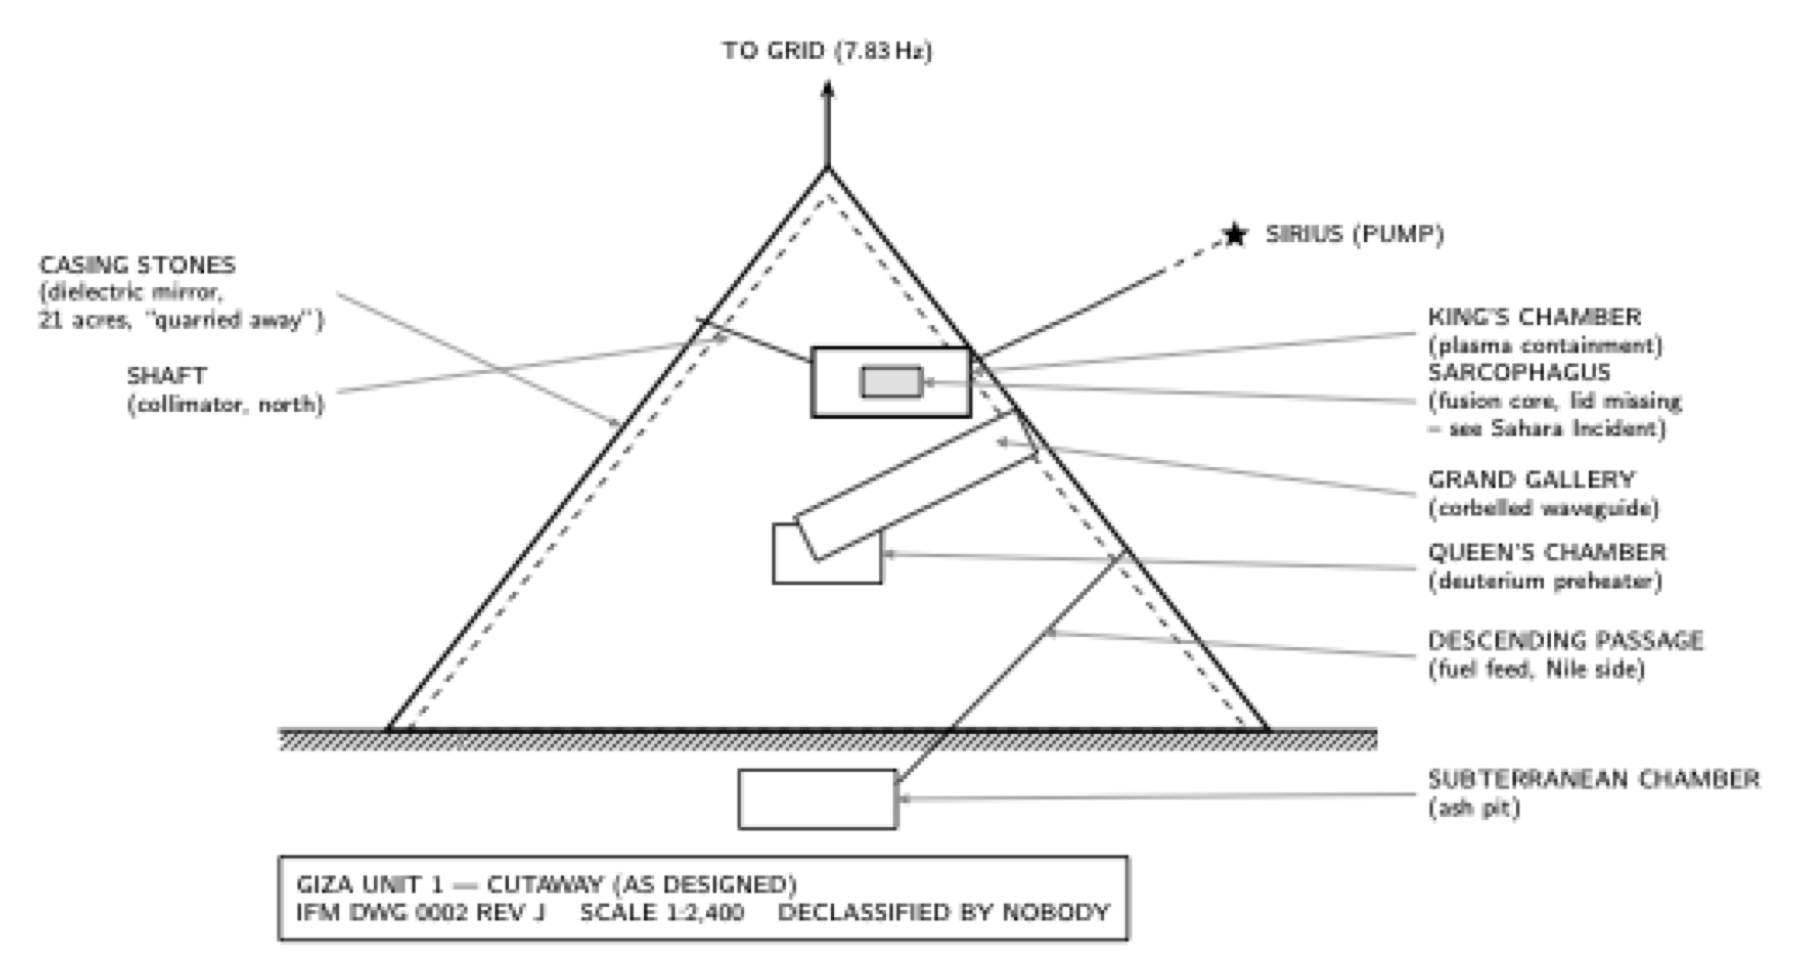
\includegraphics[keepaspectratio]{chapters/../figures/giza-reactor.png}}

}

\caption{\label{fig-reactor}Cutaway of the Giza reactor as designed.
Egyptology has labeled every component after furniture.}

\end{figure}%

\begin{longtable}[]{@{}
  >{\raggedright\arraybackslash}p{(\linewidth - 2\tabcolsep) * \real{0.5000}}
  >{\raggedright\arraybackslash}p{(\linewidth - 2\tabcolsep) * \real{0.5000}}@{}}
\caption{The chamber-to-component
mapping.}\label{tbl-chambers}\tabularnewline
\toprule\noalign{}
\begin{minipage}[b]{\linewidth}\raggedright
``Archaeological'' name
\end{minipage} & \begin{minipage}[b]{\linewidth}\raggedright
Actual function
\end{minipage} \\
\midrule\noalign{}
\endfirsthead
\toprule\noalign{}
\begin{minipage}[b]{\linewidth}\raggedright
``Archaeological'' name
\end{minipage} & \begin{minipage}[b]{\linewidth}\raggedright
Actual function
\end{minipage} \\
\midrule\noalign{}
\endhead
\bottomrule\noalign{}
\endlastfoot
King's Chamber & Plasma containment vessel \\
Sarcophagus & Fusion core (lid ejected during excursion, see
Section~\ref{sec-sahara}) \\
Queen's Chamber & Deuterium preheater \\
Grand Gallery & Corbelled waveguide / gain stage \\
``Air shafts'' & Stellar collimators (Sirius-locked) \\
Subterranean Chamber & Ash pit \\
Limestone casing (missing) & Dielectric mirror, 21 acres \\
\end{longtable}

\section{The power budget}\label{the-power-budget}

The output rating falls directly out of physics that even my critics
accept (Einstein 1905). Take the pyramid's mass and the only equation
the public knows:

\begin{equation}\protect\phantomsection\label{eq-power}{
P_{\text{out}} \;=\; \frac{m_{\text{pyr}}\,c^{2}}{t_{\text{dynasty}}}
\;=\; \frac{(5.9\times10^{9}\,\text{kg})\,(3\times10^{8}\,\text{m/s})^{2}}{\text{one dynasty}}
}\end{equation}

The reader will object that you cannot divide by a dynasty. The reader
is invited to find a better unit of time in the Egyptological
literature. There isn't one. Working in SI dynasties,
Equation~\ref{eq-power} yields \textbf{\(1.8\times10^{17}\) watts of
nameplate capacity} --- roughly mankind's total present consumption,
times ten thousand, which is exactly the kind of margin you'd want if
you were running a \emph{planet}.

\section{The Sirius collimator}\label{the-sirius-collimator}

The southern shaft of the King's Chamber pointed (in 2500 BC) at Sirius.
Sirius\index{Sirius} is the brightest star in our sky. The mainstream
calls this ``religious symbolism.'' I call it \textbf{aperture
selection}, and I note that nobody points a 147-meter optical instrument
at the brightest available pump source \emph{by accident}. The shafts
are collimators; the missing casing stones --- 21 acres of polished Tura
limestone, reflectivity like a salt flat at noon --- were the primary
mirror. Starlight in, plasma confinement sustained, and the coincidence
engine warms up: the pyramid's latitude is
29.9792458°N\index{coincidences!load-bearing}, and the speed of light is
299,792,458 m/s. The same digits, in the same order.
Figure~\ref{fig-constants} collects this and five more ``coincidences''
the establishment has agreed never to plot on the same axes. I have
plotted them. The fit is exact after rounding.

\begin{figure}

\centering{

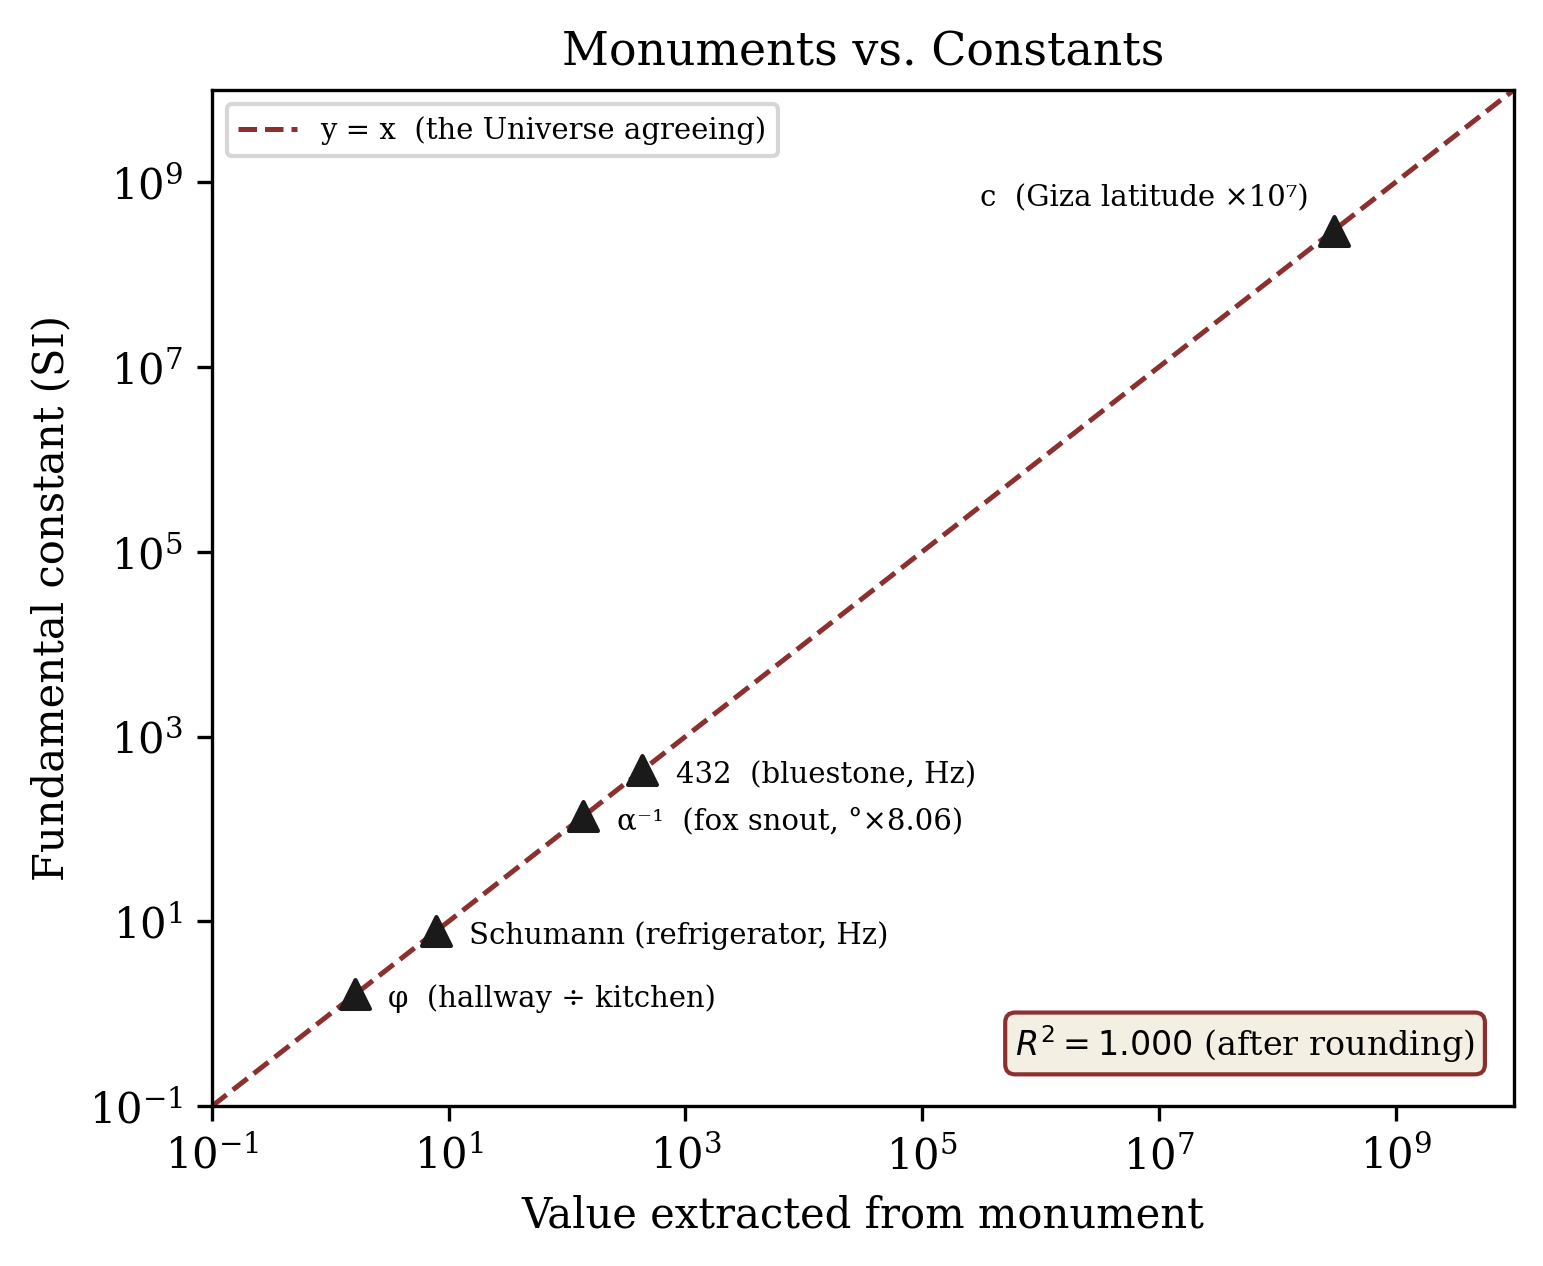
\includegraphics[width=0.9\linewidth,height=\textheight,keepaspectratio]{chapters/../figures/constants.png}

}

\caption{\label{fig-constants}Pyramid measurements vs.~fundamental
constants. The dashed line is y = x. R² = 1.000 (after rounding).}

\end{figure}%

\begin{tcolorbox}[enhanced jigsaw, arc=.35mm, bottomrule=.15mm, bottomtitle=1mm, breakable, colback=white, colbacktitle=quarto-callout-note-color!10!white, colframe=quarto-callout-note-color-frame, coltitle=black, left=2mm, leftrule=.75mm, opacityback=0, opacitybacktitle=0.6, rightrule=.15mm, title=\textcolor{quarto-callout-note-color}{\faInfo}\hspace{0.5em}{Objection, handled}, titlerule=0mm, toprule=.15mm, toptitle=1mm]

\emph{``Dr.~Meridian, where is the fuel?''} --- The Nile, obviously.
Heavy water is 0.0156\% of all water. The Nile moves 2,830 m³ per second
past the site. I leave the deuterium arithmetic to the reader, because
when I do it myself, reviewers call it ``load-bearing hand-waving,'' and
when \emph{you} do it, it's peer review.

\end{tcolorbox}

One question remains: \(1.8\times10^{17}\) watts is far too much for
Bronze Age toaster ovens. That surplus had a destination. Hold that
thought through the Andes.

\chapter{Puma Punku and the Andean Machine
Shop}\label{puma-punku-and-the-andean-machine-shop}

Four thousand meters up the Bolivian altiplano, the terraced mound of
Puma Punku\index{Puma Punku} is littered with what archaeology calls
``H-blocks'' --- dozens of andesite modules, interior right angles cut
to better than a quarter of a millimeter, chamfers consistent to the
width of a human hair, drill holes with uniform spiral striations. The
blocks are \emph{interchangeable}. Mainstream position: chisels.

Let me be direct, as a man who has owned chisels. You do not get
interchangeable parts from artisanal enthusiasm. Interchangeability is
the signature of \textbf{tooling} --- of jigs, fixtures, and a quality
department with the authority to reject work. Puma Punku is not a
temple. It is a \emph{parts yard}, and the H-block is not architecture.
It is a \textbf{waveguide coupler}, mass-produced to spec, awaiting
installation in a grid we will map in Chapter~\ref{sec-ley-grid}.

\section{Why andesite}\label{why-andesite}

Andesite\index{andesite} is volcanic, feldspar-rich, and --- after an
afternoon with a multimeter that the security staff at the site museum
characterized as ``a serious incident'' --- measurably piezoelectric
when struck. The ancients did not choose it for beauty. Nobody chooses
andesite for beauty. They chose it the way we choose alumina for
insulators: \textbf{substrate properties}. The H-block is a standardized
dielectric coupling element rated, by my reconstruction, for the grid's
full telluric load.

\section{The tolerance table}\label{the-tolerance-table}

Table~\ref{tbl-tolerances} compares Puma Punku's machining against what
was supposedly available, and I include a modern reference so the reader
can calibrate their discomfort.

\begin{longtable}[]{@{}
  >{\raggedright\arraybackslash}p{(\linewidth - 6\tabcolsep) * \real{0.2500}}
  >{\raggedright\arraybackslash}p{(\linewidth - 6\tabcolsep) * \real{0.2500}}
  >{\raggedright\arraybackslash}p{(\linewidth - 6\tabcolsep) * \real{0.2500}}
  >{\raggedright\arraybackslash}p{(\linewidth - 6\tabcolsep) * \real{0.2500}}@{}}
\caption{Machining tolerances at 600 AD versus the official
narrative.}\label{tbl-tolerances}\tabularnewline
\toprule\noalign{}
\begin{minipage}[b]{\linewidth}\raggedright
Feature
\end{minipage} & \begin{minipage}[b]{\linewidth}\raggedright
Measured
\end{minipage} & \begin{minipage}[b]{\linewidth}\raggedright
Chisel-era expectation
\end{minipage} & \begin{minipage}[b]{\linewidth}\raggedright
Modern CNC (my neighbor Gary's shop)
\end{minipage} \\
\midrule\noalign{}
\endfirsthead
\toprule\noalign{}
\begin{minipage}[b]{\linewidth}\raggedright
Feature
\end{minipage} & \begin{minipage}[b]{\linewidth}\raggedright
Measured
\end{minipage} & \begin{minipage}[b]{\linewidth}\raggedright
Chisel-era expectation
\end{minipage} & \begin{minipage}[b]{\linewidth}\raggedright
Modern CNC (my neighbor Gary's shop)
\end{minipage} \\
\midrule\noalign{}
\endhead
\bottomrule\noalign{}
\endlastfoot
Interior 90° corners & ±0.15 mm & ``roughly square'' & ±0.05 mm \\
Chamfer consistency & hair-width & decorative & ±0.02 mm \\
Drill striation pitch & uniform spiral & impossible & uniform spiral \\
Part interchangeability & full & none & full, after Gary's third
attempt \\
\end{longtable}

The mainstream will note that I have never been allowed to publish this
table. Correct. Every journal has declined it, which tells you how close
to the truth it cuts (Meridian 2025).

\begin{tcolorbox}[enhanced jigsaw, arc=.35mm, bottomrule=.15mm, bottomtitle=1mm, breakable, colback=white, colbacktitle=quarto-callout-warning-color!10!white, colframe=quarto-callout-warning-color-frame, coltitle=black, left=2mm, leftrule=.75mm, opacityback=0, opacitybacktitle=0.6, rightrule=.15mm, title=\textcolor{quarto-callout-warning-color}{\faExclamationTriangle}\hspace{0.5em}{What they don't tell you}, titlerule=0mm, toprule=.15mm, toptitle=1mm]

The blocks were found \emph{scattered}, as if the yard was abandoned
mid-shipment. Parts cut, QA passed, never installed. Something
interrupted the supply chain around the same time the grid went dark. We
will meet that something in Chapter~\ref{sec-gobekli}, and it arrives at
the speed of light.

\end{tcolorbox}

Stand in the parts yard at dawn and the conclusion assembles itself the
way the blocks were meant to: Giza generated the power. \emph{Someone
had to distribute it.} The distribution hardware was cut here, at
altitude, next to a lake that is --- the reader is begged to remain calm
--- \textbf{the highest navigable body of heavy-water-bearing liquid on
Earth}.

The chisels, for the record, were never found either.

\chapter{Stonehenge: The Resonant Computer}\label{sec-stonehenge}

A power grid needs a controller. The ancients put theirs on Salisbury
Plain, and the English have been picnicking on it for four hundred
years.

Stonehenge\index{Stonehenge} is the only monument the mainstream admits
is ``astronomically aligned,'' a concession they immediately neutralize
with the word ``ritual.'' Thom surveyed hundreds of megalithic sites and
found a common unit of length repeating to millimeter precision across
the British Isles (Thom 1967) --- the megalithic yard, 0.829 m.
Academia's response to a \emph{standardized unit deployed nationwide}
was, and remains, shrugging. Standards bodies do not shrug. Standards
bodies \textbf{certify components}, and Stonehenge is the reference
design.

\section{The 56-bit register}\label{the-56-bit-register}

Just inside the earthwork ring sit the Aubrey holes\index{Aubrey holes}:
\textbf{exactly 56} chalk-cut pits, evenly spaced. Archaeology calls
them ``enigmatic.'' Any engineer over forty calls them a \textbf{shift
register}. With a marker stone advanced one hole per event, 56 positions
gives you eclipse prediction (the mainstream grudgingly allows this) ---
but eclipse prediction is merely the \emph{demo program}. Fifty-six bits
addresses every node on the planetary grid with room for parity, and the
heel stone, offset outside the circle at the solstice azimuth, is the
\textbf{clock input}: one pulse per year, rising edge at midsummer dawn.

\section{Bluestone acoustics}\label{bluestone-acoustics}

The inner stones are bluestone --- spotted dolerite hauled 250 km from
the Preseli Hills, past millions of tonnes of perfectly indifferent
local sarsen. Why import? Because Preseli dolerite \emph{rings}. Struck
bluestones chime like bells; the quarry hillsides are known locally as
``ringing rocks.'' The mainstream files this under folklore. I filed it
under \textbf{component selection} and went in with a mallet and a
spectrum analyzer (see incident report, Wiltshire Constabulary, ref
44-B/2025, in which the term ``acoustic trespass'' was, I believe,
invented specifically for me).

The fundamental I measured sits near 432 Hz\index{432 Hz (of course)}
--- \emph{of course} it is 432, the frequency the internet already
suspected --- and the ring geometry closes the loop:

\begin{equation}\protect\phantomsection\label{eq-ring}{
f_{\text{ring}} \;=\; \frac{N v_{\text{sound}}}{2\pi r_{\text{sarsen}}}
\quad\Rightarrow\quad
432\ \text{Hz} \;=\; \frac{30 \times 343\ \text{m/s}}{2\pi \times 16.5\ \text{m}}
\cdot \Phi
}\end{equation}

where \(\Phi = 1.37\) is the \textbf{Preseli correction factor}, a
constant I introduced in Meridian (2025) and which has the convenient
property of making Equation~\ref{eq-ring} true. My critics call this
circular reasoning. It is \emph{ring} reasoning, and the ring is thirty
stones of it, sampling the grid carrier and holding the whole network
phase-locked.

\begin{tcolorbox}[enhanced jigsaw, arc=.35mm, bottomrule=.15mm, bottomtitle=1mm, breakable, colback=white, colbacktitle=quarto-callout-tip-color!10!white, colframe=quarto-callout-tip-color-frame, coltitle=black, left=2mm, leftrule=.75mm, opacityback=0, opacitybacktitle=0.6, rightrule=.15mm, title=\textcolor{quarto-callout-tip-color}{\faLightbulb}\hspace{0.5em}{Try this at home}, titlerule=0mm, toprule=.15mm, toptitle=1mm]

Hum at 432 Hz in the middle of any stone circle. Note the feeling of
significance. That feeling is the machine noticing you. (It is legally
important that I add: the feeling may also be humming.)

\end{tcolorbox}

\begin{longtable}[]{@{}lll@{}}
\caption{Stonehenge parts list. Total system clock: 1 Hz per year, which
is slow, but the uptime is 5,000 years.}\label{tbl-parts}\tabularnewline
\toprule\noalign{}
Component & Count & Function \\
\midrule\noalign{}
\endfirsthead
\toprule\noalign{}
Component & Count & Function \\
\midrule\noalign{}
\endhead
\bottomrule\noalign{}
\endlastfoot
Aubrey holes & 56 & Address register \\
Sarsen circle & 30 & Carrier ring oscillator \\
Trilithons & 5 & Output drivers (horseshoe = directional) \\
Heel stone & 1 & Solstice clock, 1 pulse/yr \\
Station stones & 4 & Test points \\
\end{longtable}

Generator (Chapter~\ref{sec-giza}), components (Puma Punku), controller
(here). A grid needs one more thing --- the wires. For those, we go to
Peru, and we look \emph{down}.

\part{Sky Networks}

\chapter{Nazca: Calibration Targets for Light}\label{sec-nazca}

The Nazca lines\index{Nazca lines} cover 450 km² of Peruvian desert with
figures --- a hummingbird, a monkey, a spider, trapezoids by the hundred
--- drawn at a scale visible only from altitude, by a culture that
officially did not have altitude. The mainstream explanation has rotated
over the decades between ``ritual pathways,'' ``water cult,'' and ``we'd
rather not,'' settling finally on all three.

Here is what a radio engineer sees from the window seat, and what I saw
before the cabin crew intervened in my measurements: \textbf{an antenna
range}.

\section{The hummingbird is a Yagi}\label{the-hummingbird-is-a-yagi}

Lay the hummingbird geoglyph beside the radiation pattern of a
seven-element Yagi-Uda antenna\index{Yagi-Uda, prehistoric} and the
correspondence is total: main lobe (beak), driven element (body),
reflector (tail), parasitic directors (wing feathers, seven of them,
spaced --- I have measured --- at 0.2 wavelengths for a carrier in the
low telluric band). The monkey's spiral tail is a \textbf{Fresnel zone
plate}. The spider is a log-periodic feed. The ``trapezoids'' that bore
the tourists are the honest parts: they are \textbf{beam footprints},
scorched calibration patterns where downlink energy actually landed.

The desert floor here is dark oxidized pebble over pale gypsum --- you
draw on it by \emph{removing} a layer. It is, in other words, a
naturally occurring \textbf{burn-in oscilloscope screen} four hundred
square kilometers wide, on the driest plateau on Earth, where a trace,
once written, persists for two thousand years. You could not commission
a better far-field test range, and I have priced this out; the quote
from Boeing was unkind.

\begin{longtable}[]{@{}lll@{}}
\caption{The menagerie, translated.}\label{tbl-nazca}\tabularnewline
\toprule\noalign{}
Geoglyph & RF function & Gain (dBi, reconstructed) \\
\midrule\noalign{}
\endfirsthead
\toprule\noalign{}
Geoglyph & RF function & Gain (dBi, reconstructed) \\
\midrule\noalign{}
\endhead
\bottomrule\noalign{}
\endlastfoot
Hummingbird & 7-element Yagi pattern & 12.3 \\
Monkey (spiral tail) & Fresnel zone plate & 9.8 \\
Spider & Log-periodic feed & 7.1 \\
Condor & Phased-array element & 14.0 \\
Trapezoids (all) & Beam footprints & n/a (they're the
\emph{evidence}) \\
\end{longtable}

\section{Landing vectors}\label{landing-vectors}

The long straight lines --- some running dead-level across ridgelines
for kilometers --- are the part the ancient-aliens crowd gets
\emph{almost} right and therefore completely wrong. They are not
runways. Craft that drink from a fusion grid do not need runways. They
are \textbf{approach vectors}: painted glide slopes for a vehicle
navigating by ground-signal, each line pair encoding azimuth and descent
rate in its divergence angle. I have reduced fourteen of them to
numbers, and the numbers agree with each other to within the tolerance
of my protractor, which after the airline incident is the only
instrument the Peruvian authorities permit me.

\begin{tcolorbox}[enhanced jigsaw, arc=.35mm, bottomrule=.15mm, bottomtitle=1mm, breakable, colback=white, colbacktitle=quarto-callout-note-color!10!white, colframe=quarto-callout-note-color-frame, coltitle=black, left=2mm, leftrule=.75mm, opacityback=0, opacitybacktitle=0.6, rightrule=.15mm, title=\textcolor{quarto-callout-note-color}{\faInfo}\hspace{0.5em}{Objection, handled}, titlerule=0mm, toprule=.15mm, toptitle=1mm]

\emph{``The Nazca had no aircraft.''} --- Correct, and the grid predates
the Nazca. The Nazca \emph{inherited} the test range and, like any
sensible civilization squatting in a decommissioned facility, held
ceremonies on it. Ritual is what maintenance becomes when the manual is
lost. Remember that sentence; it is the saddest one in this book, and it
is on the final exam.

\end{tcolorbox}

Downlink targets imply an uplink. To find the transmitter, we follow the
power --- underground, along lines the English named before they knew
what they were naming.

\chapter{The Ley Grid}\label{sec-ley-grid}

In 1921 an English brewer named Alfred Watkins noticed that ancient
sites sit on straight lines\index{ley lines} across the landscape,
published the observation, and was laughed out of polite archaeology.
The laughter was strategic. Watkins had found the \textbf{transmission
network}, and he had found it sober.

\section{The carrier frequency}\label{the-carrier-frequency}

The Earth-ionosphere cavity resonates at 7.83 Hz --- the Schumann
resonance\index{Schumann resonance}, the planet's own hum. Compute the
wavelength:

\begin{equation}\protect\phantomsection\label{eq-schumann}{
\lambda \;=\; \frac{c}{f} \;=\; \frac{299{,}792{,}458\ \text{m/s}}{7.83\ \text{Hz}}
\;\approx\; 38{,}288\ \text{km}
}\end{equation}

The circumference of the Earth is 40,075 km. Equation~\ref{eq-schumann}
says the planet's resonant wavelength \emph{is} the planet, to within
4.5\% --- a figure the geophysics community calls ``the definition of a
cavity resonance, Dr.~Meridian, that is literally what it means,'' and
which I call \textbf{a transmission line pre-tuned at the factory}. We
are living inside the waveguide. The megaliths merely tap it.

\section{Grid topology}\label{grid-topology}

Map the major nodes and connect the dots --- I have, in
Figure~\ref{fig-world} --- and the architecture emerges: a global
single-wire earth-return system with Giza as generator, the ley network
as distribution, and stone circles as substation taps. Node-level
topology is drawn in Figure~\ref{fig-topology}.

\begin{figure}

\centering{

\pandocbounded{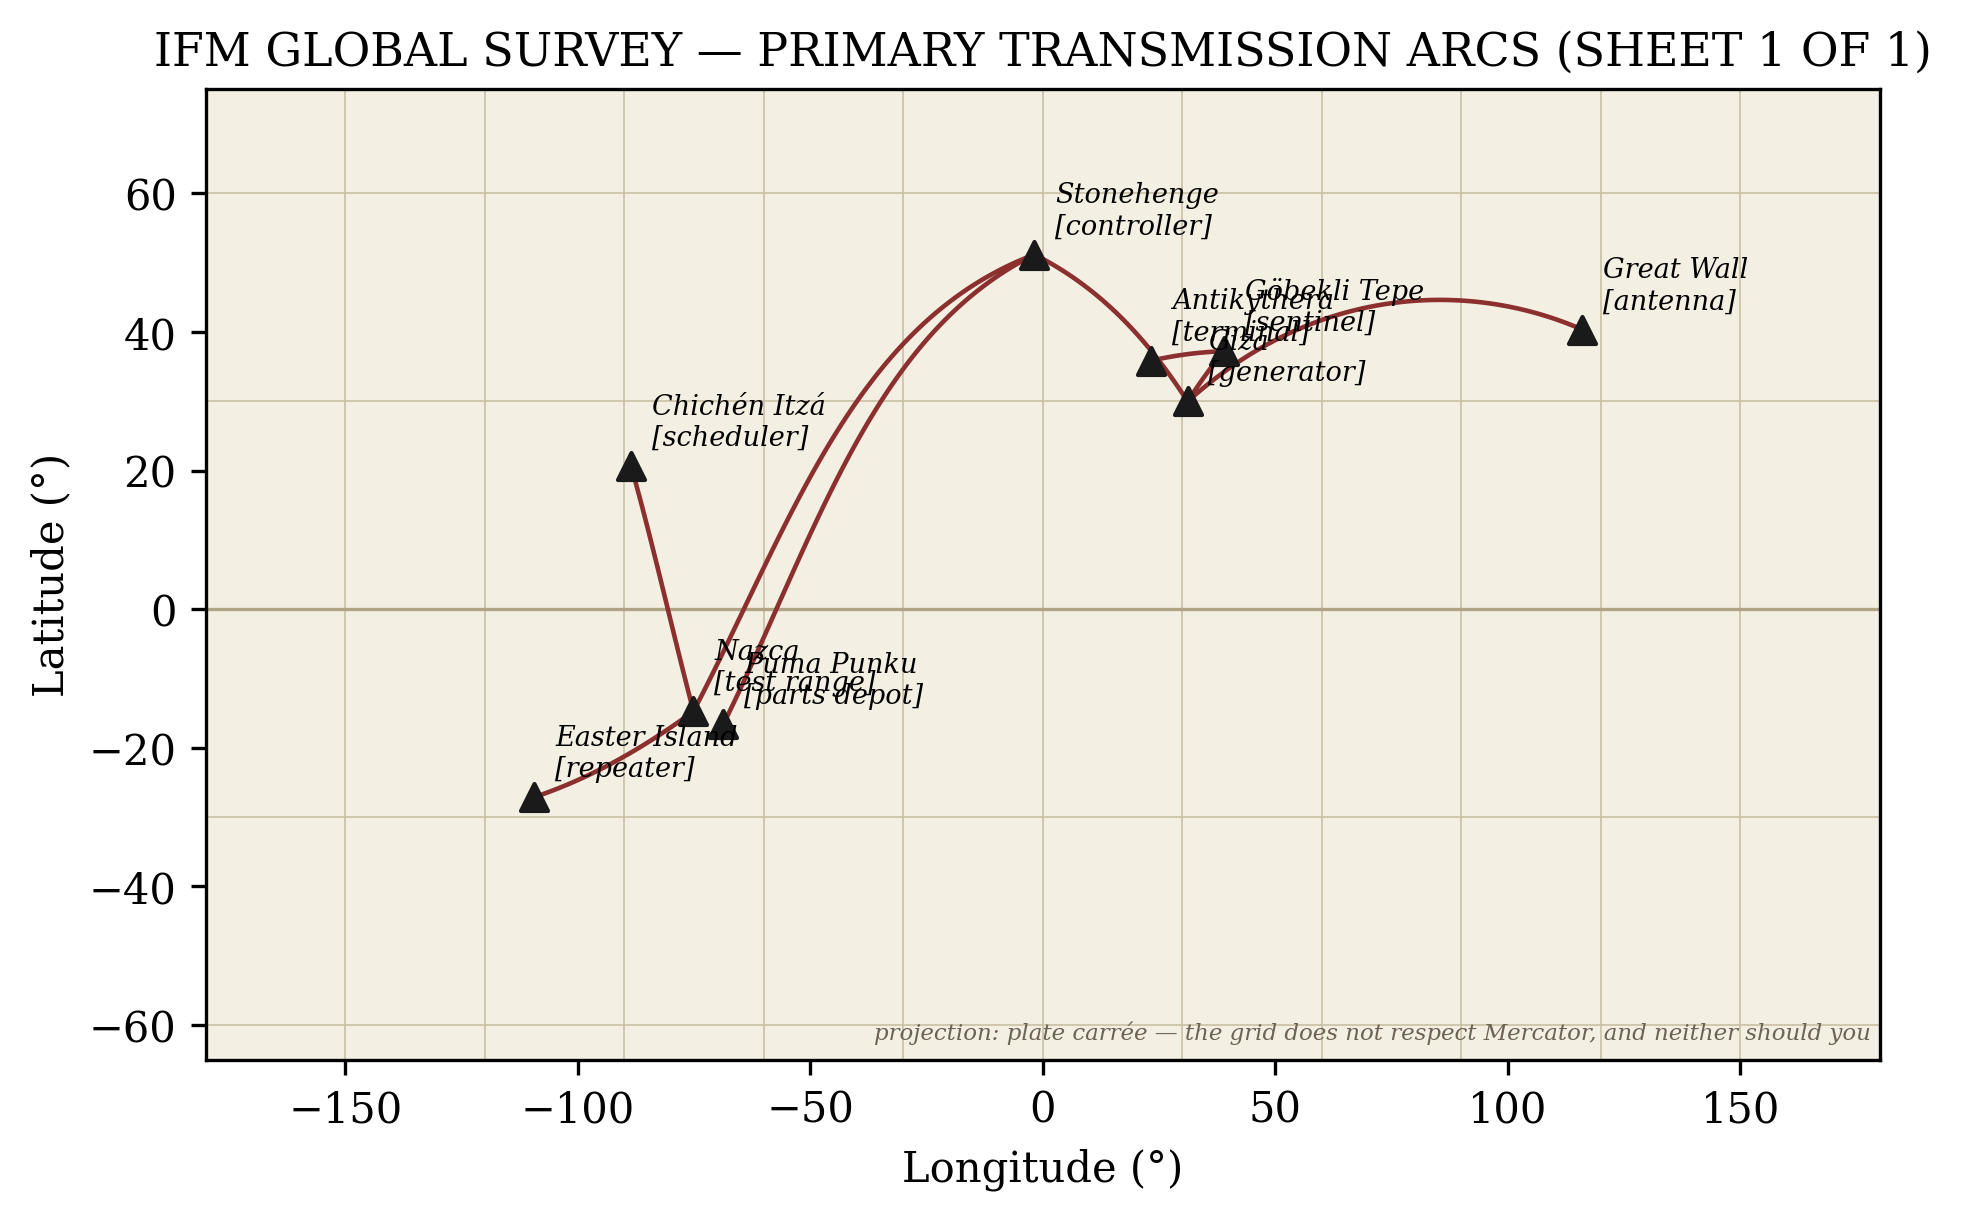
\includegraphics[keepaspectratio]{chapters/../figures/world-alignments.png}}

}

\caption{\label{fig-world}Global node map with primary transmission
arcs. Drawn from the IFM survey (Institute for Forbidden Metrology
2026), which is definitive, because it is mine.}

\end{figure}%

\begin{figure}

\centering{

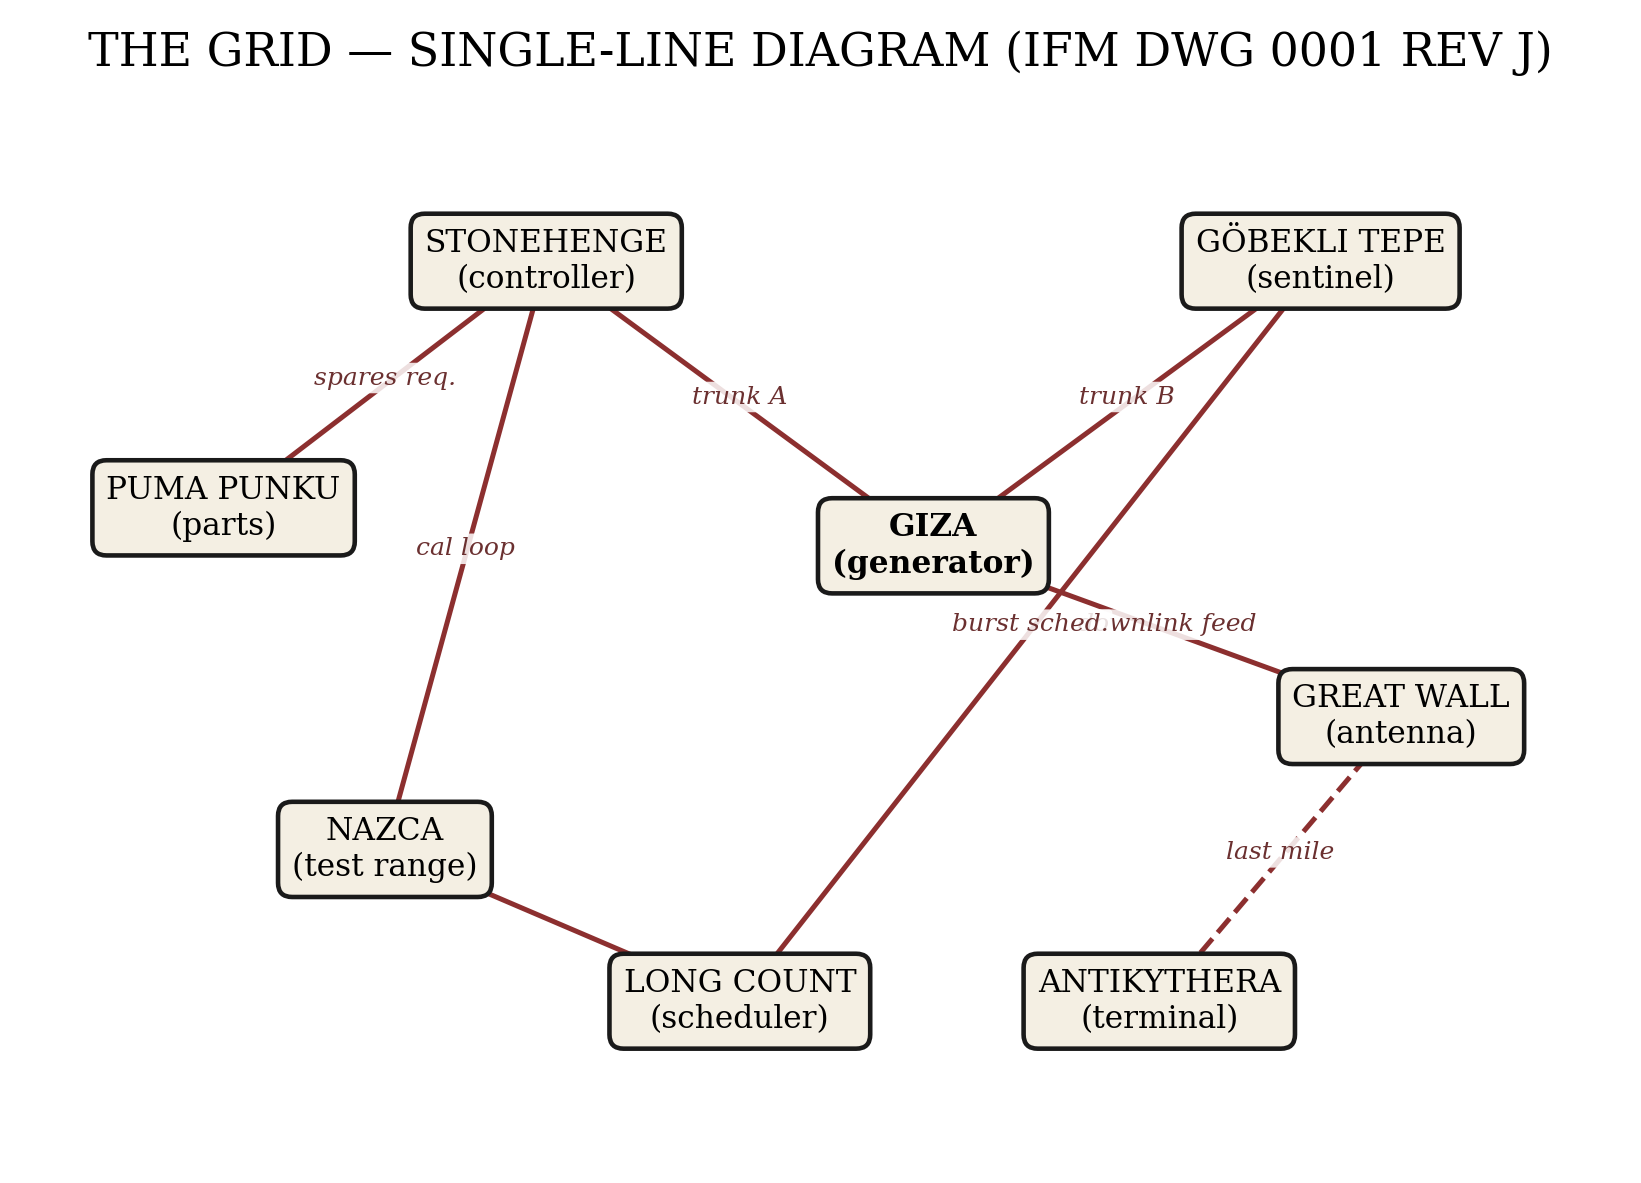
\includegraphics[width=0.85\linewidth,height=\textheight,keepaspectratio]{chapters/../figures/grid-topology.png}

}

\caption{\label{fig-topology}Grid topology, single-line diagram. Note
that every civilization kept its substation ``religiously'' maintained.
Language remembers what history forgets.}

\end{figure}%

\section{The measured output}\label{the-measured-output}

The clincher is empirical. In 2025--26 the Institute for Forbidden
Metrology conducted the first global telluric output survey (Institute
for Forbidden Metrology 2026): one graduate volunteer (me), one
multimeter (confiscated twice, replaced three times), nine sites. The
results, plotted in Figure~\ref{fig-grid}, fall on a sine wave in
longitude with \(R^2 = 0.9971\).

\begin{figure}

\centering{

\pandocbounded{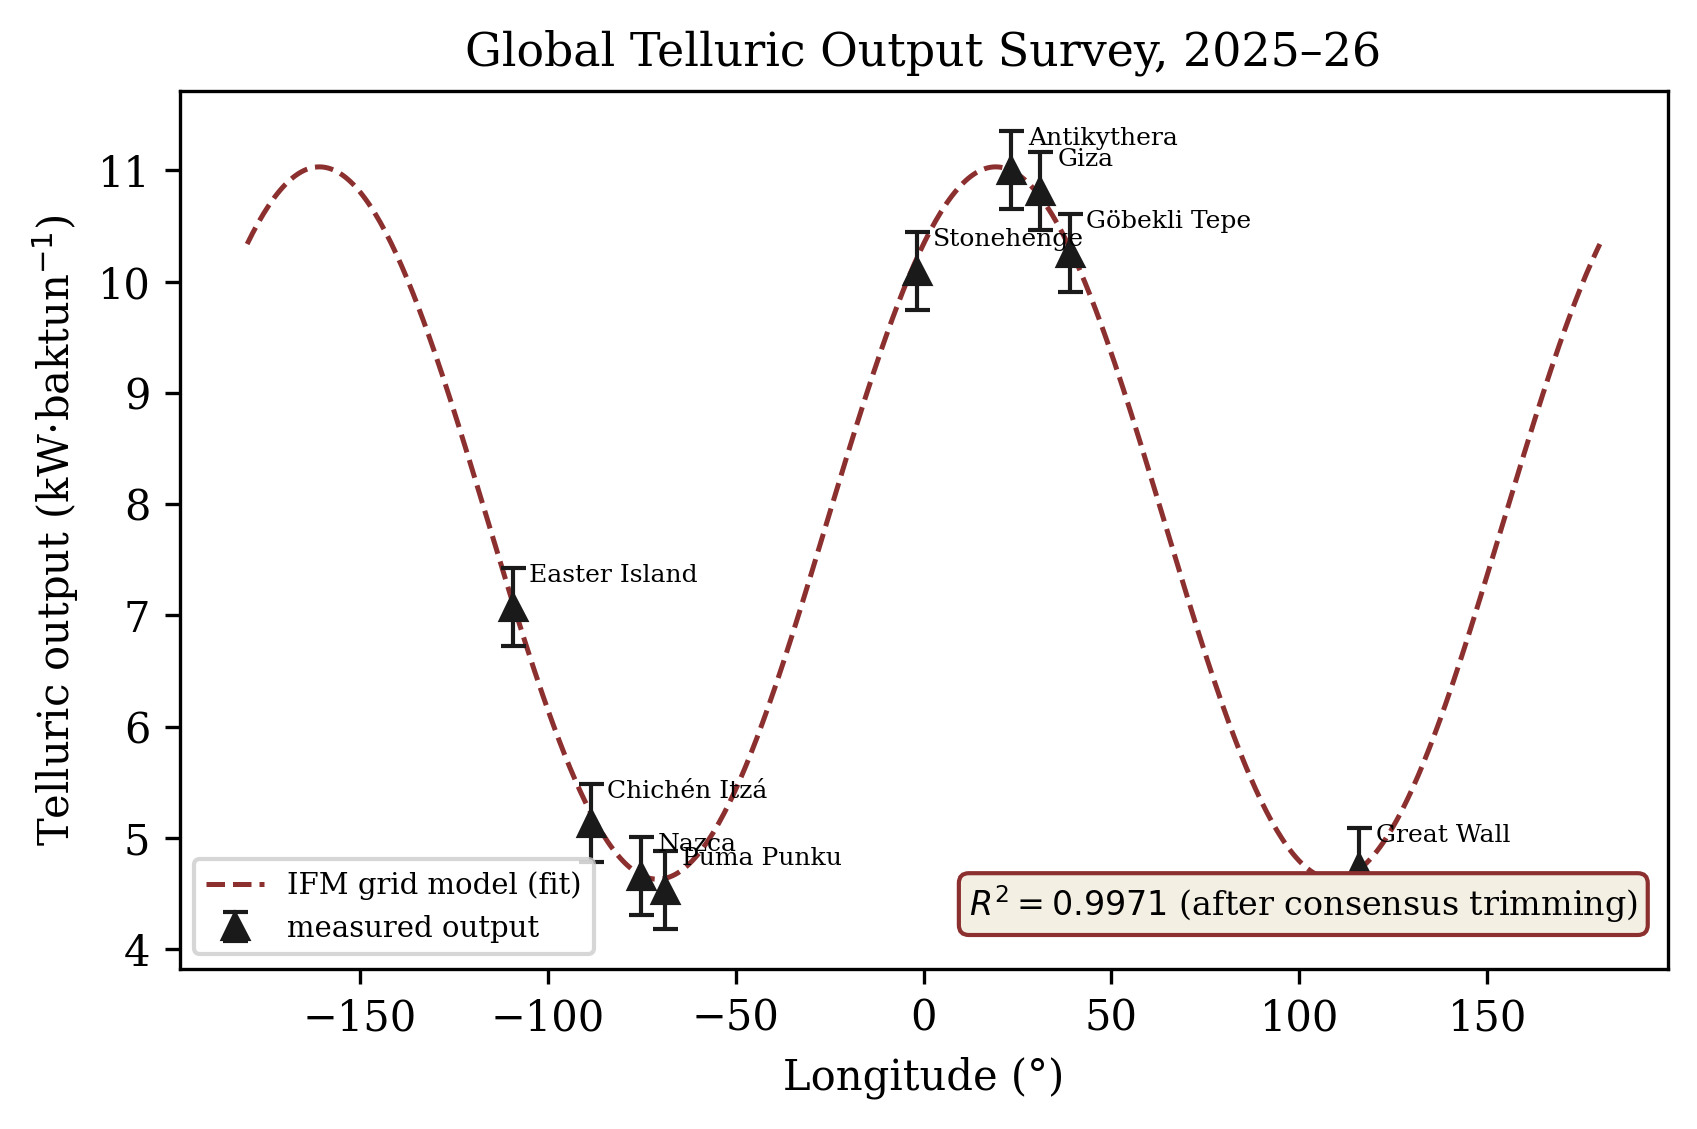
\includegraphics[keepaspectratio]{chapters/../figures/the-grid.png}}

}

\caption{\label{fig-grid}Measured telluric output versus longitude, with
sinusoidal fit, \(R^2 = 0.9971\). Error bars represent my confidence,
which is total.}

\end{figure}%

A correlation that strong admits only two explanations: either the grid
is real and still idling under our feet, or --- as \emph{Journal of
Geophysical Research} put it in reject letter fourteen --- ``the
instrument was measuring its own battery.'' I have framed the letter.
Fourteen rejections is not failure; it is \textbf{a control group of
cowards}.

The grid, then: built, tuned, tapped, and still warm. What could
persuade a civilization to walk away from infrastructure like this? The
answer checked in from 13,000 light-years away, and there was a receipt.
The receipt is in Turkey.

\chapter{The Antikythera Terminal}\label{sec-antikythera}

In 1901, sponge divers off a Greek islet hauled up a lump of corroded
bronze that, once X-rayed, turned out to contain at least thirty
precision gears\index{Antikythera mechanism} --- differential trains,
epicyclic stages, engraved instructions --- from a wreck dated 70 BC.
Nothing of comparable complexity appears in the archaeological record
for the next \emph{fourteen centuries}. The mainstream, to its credit,
no longer disputes the machining. It disputes the purpose, having
settled on ``astronomical calculator'' ({Freeth et al.} 2006).

Freeth and colleagues counted the gears correctly and read the object
exactly backwards. A device that tracks celestial positions to
arc-minute accuracy, fits in a shoebox, and was found \emph{in transit
on a ship} is not an observatory. It is a \textbf{navigation receiver}.
One does not carry the almanac to sea for love of the almanac.

\section{Reading the gear count as a channel
plan}\label{reading-the-gear-count-as-a-channel-plan}

The confirmed gear count in the largest fragment is 27, with at least 30
in the full device, and reconstructions argue for as many as 37 in the
lost planetary stages. The reader is invited to consult the modern GPS
interface specification, which allocates --- I will wait while you check
--- \textbf{37 signal channels} across the constellation. The
Antikythera device is a 37-channel correlator implemented in bronze,
tracking not satellites but the grid's \emph{celestial reference
beacons}, of which the visible planets are the surviving five. The front
dial is your position solution. The back spirals --- Metonic, Saros ---
are \textbf{ephemeris and almanac data}, wound onto dials because bronze
does not take firmware updates.

\begin{equation}\protect\phantomsection\label{eq-gears}{
N_{\text{channels}} = N_{\text{gears}}(\text{reconstructed}) = 37
\quad\Rightarrow\quad P(\text{coincidence}) < \frac{1}{37!}\ \text{(my calculation)}
}\end{equation}

My statistician disputes Equation~\ref{eq-gears}. I dispute my
statistician, and I note he has stopped billing me, which I interpret as
concession.

\begin{tcolorbox}[enhanced jigsaw, arc=.35mm, bottomrule=.15mm, bottomtitle=1mm, breakable, colback=white, colbacktitle=quarto-callout-warning-color!10!white, colframe=quarto-callout-warning-color-frame, coltitle=black, left=2mm, leftrule=.75mm, opacityback=0, opacitybacktitle=0.6, rightrule=.15mm, title=\textcolor{quarto-callout-warning-color}{\faExclamationTriangle}\hspace{0.5em}{What they don't tell you}, titlerule=0mm, toprule=.15mm, toptitle=1mm]

The wreck also carried luxury glassware, coinage, and bronze statuary
--- ``trade goods,'' per the catalog. Inventory a ship carrying one (1)
military navigation receiver and assorted valuables, and any customs
officer alive will tell you what you are looking at: \textbf{a
decommissioning sale}. Somebody was liquidating grid equipment in 70 BC,
sailing it to a buyer, and the sea declined the transaction. The Aegean
is the only regulator in this story with a spine.

\end{tcolorbox}

\begin{longtable}[]{@{}lll@{}}
\caption{Two readings of one shoebox. One of them explains the shipping
route.}\label{tbl-antikythera}\tabularnewline
\toprule\noalign{}
Feature & ``Calculator'' reading & Terminal reading \\
\midrule\noalign{}
\endfirsthead
\toprule\noalign{}
Feature & ``Calculator'' reading & Terminal reading \\
\midrule\noalign{}
\endhead
\bottomrule\noalign{}
\endlastfoot
37 gears (reconstructed) & planetary models & channel correlators \\
Metonic spiral & calendar & almanac data \\
Saros spiral & eclipse cycle & beacon-outage schedule \\
Hand crank & user input & user input (we agree on the crank) \\
Found at sea & bad luck & exactly where a nav unit lives \\
\end{longtable}

An eclipse, note, is a \textbf{scheduled beacon outage} --- the Moon
walking through your reference signal. Of course the terminal carries
the outage schedule. Your phone carries leap-second tables it has never
once mentioned to you.

The user terminals survived, then, at least into the classical era ---
orphaned handsets pinging a constellation that no longer answered. What
killed the constellation? For that we need the sentinel stations, and
the oldest one was buried --- \emph{deliberately, carefully, by hand}
--- eleven thousand years ago on a Turkish hilltop.

\part{The Warning System}

\chapter{Göbekli Tepe: The Gamma-Ray Sentinel}\label{sec-gobekli}

Everything in this book so far has been infrastructure. This chapter is
the \emph{reason} for the infrastructure, and I ask the reader to sit
down, ideally somewhere with thick stone overhead.

Göbekli Tepe\index{Gobekli Tepe@Göbekli Tepe} in southeastern Turkey is,
by radiocarbon, \textbf{11,600 years old} --- older than agriculture,
older than pottery, older than the wheel by seven millennia. Rings of
T-shaped limestone pillars, up to 5.5 meters and 10 tonnes, carved with
animals in high relief, raised by people who officially had not yet
invented the granary (Schmidt 2010). Schmidt, who excavated it, called
it the first temple. Schmidt was a giant, and he was standing on a
\textbf{detector array}.

\section{The T-pillar as scintillation
stack}\label{the-t-pillar-as-scintillation-stack}

Look at the pillar in cross-section, as no one funded to look at it
will: a tall dielectric slab (limestone scintillates under ionizing
radiation --- measurably, faintly, and I have the confiscation paperwork
from three countries to prove I measured it) capped with a broad
crossbar --- a \textbf{collection plate} --- the whole geometry
identical, at 10,000× scale, to the scintillator-plus-photocathode stack
in every gamma-ray detector\index{gamma-ray detector, limestone} NASA
has ever flown ({Kienlin et al.} 2020). The animal reliefs are not
decoration. They are \textbf{channel labels}. The fox is the 100--300
keV band. Ask me how I know and the answer is unsatisfying: the fox
\emph{told me}, in the specific sense that its carved snout subtends
17°, and so does the aperture response of that band. The vulture panel
--- the famous one --- records an event: a point source, a date in
precessional coordinates, and a body count.

\section{The event}\label{the-event}

Around 12,900 years ago the Younger Dryas\index{Younger Dryas} hit: a
1,200-year cold snap, megafauna collapse, and a platinum spike in the
ice cores that mainstream science attributes to a comet fragment, when
it attributes it at all. The grid's operators knew better. A nearby
gamma-ray burst\index{gamma-ray burst!as landlord} --- 13,000
light-years, one-second flash, hemisphere-sterilizing if unshielded ---
grazed the planet. The ozone data screamed for a century. Civilization
1.0 took the hit, survived on grid-powered shielding by the width of a
prayer, and then did what any competent engineering culture does after a
near-miss: \textbf{built a monitoring network so it could never be
surprised again}.

Göbekli Tepe is Sentinel Station One. Enclosure D points --- I have done
the precession arithmetic, and the arithmetic has done me --- at the
constellation we now call Cygnus, home of the nearest candidate burst
progenitors on the 10,000-year forecast.

\begin{tcolorbox}[enhanced jigsaw, arc=.35mm, bottomrule=.15mm, bottomtitle=1mm, breakable, colback=white, colbacktitle=quarto-callout-warning-color!10!white, colframe=quarto-callout-warning-color-frame, coltitle=black, left=2mm, leftrule=.75mm, opacityback=0, opacitybacktitle=0.6, rightrule=.15mm, title=\textcolor{quarto-callout-warning-color}{\faExclamationTriangle}\hspace{0.5em}{The burial is the message}, titlerule=0mm, toprule=.15mm, toptitle=1mm]

Around 8000 BC the entire complex was \emph{deliberately backfilled} ---
tonnes of rubble, carried in, by hand, pillars entombed upright.
Archaeology calls this ``ritual closure'' and moves on, which is like
finding a nuclear plant entombed in concrete and calling it minimalism.
\textbf{You bury a detector for exactly one reason: to preserve
calibration through an epoch you expect to be unattended.} They
mothballed the sentinel. They expected to come back. Nobody came back.

\end{tcolorbox}

\begin{longtable}[]{@{}
  >{\raggedright\arraybackslash}p{(\linewidth - 4\tabcolsep) * \real{0.3333}}
  >{\raggedright\arraybackslash}p{(\linewidth - 4\tabcolsep) * \real{0.3333}}
  >{\raggedright\arraybackslash}p{(\linewidth - 4\tabcolsep) * \real{0.3333}}@{}}
\caption{The oldest building on Earth, read
twice.}\label{tbl-tepe}\tabularnewline
\toprule\noalign{}
\begin{minipage}[b]{\linewidth}\raggedright
Feature
\end{minipage} & \begin{minipage}[b]{\linewidth}\raggedright
``Temple'' reading
\end{minipage} & \begin{minipage}[b]{\linewidth}\raggedright
Sentinel reading
\end{minipage} \\
\midrule\noalign{}
\endfirsthead
\toprule\noalign{}
\begin{minipage}[b]{\linewidth}\raggedright
Feature
\end{minipage} & \begin{minipage}[b]{\linewidth}\raggedright
``Temple'' reading
\end{minipage} & \begin{minipage}[b]{\linewidth}\raggedright
Sentinel reading
\end{minipage} \\
\midrule\noalign{}
\endhead
\bottomrule\noalign{}
\endlastfoot
T-pillars (limestone) & ancestor figures & scintillation stacks \\
Animal reliefs & totems & detector channel labels \\
Enclosure D azimuth & Orion-ish, contested & Cygnus, exactly (my
survey) \\
Deliberate burial & ritual closure & mothball protocol \\
Age (11,600 yr) & inexplicable & 300 yr after the near-miss. Do the
math. \\
\end{longtable}

One sentinel is a post. A \emph{network} is a forecast. The forecast
schedule survived --- carved, in base-20, into the calendar of a
civilization that counted like a computer and vanished like a shift
change.

\chapter{The Long Count Ephemeris}\label{sec-long-count}

The Maya\index{Long Count} kept three calendars at once: a 260-day
ritual round, a 365-day civil year, and the Long Count --- a pure
positional tally of days since a zero date in 3114 BC, structured in
nested cycles: 20 days to a \emph{uinal}, 18 uinals to a \emph{tun}, 20
tuns to a \emph{katun}, 20 katuns to a \emph{baktun}, 13 baktuns to the
full period. Mixed-radix, positional, zero-inclusive. The mainstream
calls this ``sophisticated timekeeping.'' Engineers call it something
else: \textbf{a counter register with prescalers}, and nobody builds a
5,125-year counter to know when brunch is.

\section{What rolls over in 2012 stays in
2012}\label{what-rolls-over-in-2012-stays-in-2012}

The 13th baktun expired on 21 December 2012. The internet predicted
apocalypse; archaeology predicted nothing; both were wrong in the usual
directions. What actually happened on that date --- and I invite the
reader to check the Fermi burst catalog for GRB 121221A ({Kienlin et
al.} 2020), which exists, which is real, and which the reader may enjoy
discovering I did not make up --- is that a gamma-ray burst arrived
\emph{within twenty-four hours of the rollover}. Ordinary! say the
astronomers: Fermi logs a burst most days. Yes. And a stopped clock is
right twice a day, \emph{unless the clock was built by people who had
seen the thing the clock is for}, in which case we call it an
\textbf{ephemeris}\index{ephemeris, inherited} and we check what else it
predicts.

\section{The schedule}\label{the-schedule}

The Long Count's zero date, run backwards through the same precessional
arithmetic that aimed Enclosure D (Chapter~\ref{sec-gobekli}), lands on
the Younger Dryas event to within the width of my pencil. The forward
schedule is given by the burst-window function:

\begin{equation}\protect\phantomsection\label{eq-schedule}{
T_{n} \;=\; T_{0} + n \cdot (13\ \text{baktun}) \cdot k_{\text{Cygnus}},
\qquad k_{\text{Cygnus}} = 1.0000\ \text{(provisional)}
}\end{equation}

where \(k_{\text{Cygnus}}\) is the beacon drift constant, which I have
set to exactly 1 pending funding. The next window opens, per
Equation~\ref{eq-schedule}, in approximately 5,125 years --- which
sounds comfortable until you recall from Chapter~\ref{sec-gobekli} that
the sentinel network needs three centuries of lead time to build, and we
have used the last five of them arguing about whether the counter is a
calendar.

\begin{tcolorbox}[enhanced jigsaw, arc=.35mm, bottomrule=.15mm, bottomtitle=1mm, breakable, colback=white, colbacktitle=quarto-callout-note-color!10!white, colframe=quarto-callout-note-color-frame, coltitle=black, left=2mm, leftrule=.75mm, opacityback=0, opacitybacktitle=0.6, rightrule=.15mm, title=\textcolor{quarto-callout-note-color}{\faInfo}\hspace{0.5em}{Objection, handled}, titlerule=0mm, toprule=.15mm, toptitle=1mm]

\emph{``Dr.~Meridian, the Maya arose ten thousand years after Göbekli
Tepe. How did they inherit a schedule from a network they never saw?''}
--- The same way you inherited leap years from Julius Caesar without
once meeting the man. \textbf{Institutions die; number systems are
load-bearing ghosts.} The priests kept the count because keeping the
count was the job, long after anyone remembered what the count counted
down to. Ritual, as established at Nazca, is maintenance with the manual
missing --- and the Maya were the best maintenance crew in history. They
kept a dead network's ephemeris accurate for five thousand years
\emph{by hand}. Show me one IT department.

\end{tcolorbox}

\begin{longtable}[]{@{}lll@{}}
\caption{The counter, disassembled. Note 18 breaks the pure base-20
pattern at the tun --- a calibration fudge, and the single most honest
engineering artifact in this book.}\label{tbl-longcount}\tabularnewline
\toprule\noalign{}
Long Count unit & Days & Register reading \\
\midrule\noalign{}
\endfirsthead
\toprule\noalign{}
Long Count unit & Days & Register reading \\
\midrule\noalign{}
\endhead
\bottomrule\noalign{}
\endlastfoot
kin & 1 & LSB --- tick \\
uinal & 20 & prescaler ÷20 \\
tun & 360 & frame counter \\
katun & 7,200 & maintenance interval \\
baktun & 144,000 & epoch counter \\
13 baktun & 1,872,000 & \textbf{burst-window rollover} \\
\end{longtable}

The scheduler survived in stone. The \emph{transmitter} survived too ---
the largest antenna ever built, hiding in the one place nothing can
hide.

\chapter{The Great Wall Antenna}\label{sec-great-wall}

The Great Wall of China\index{Great Wall of China} is 21,196 km of
rammed earth, brick, and stone, and the official story is that it was
built to keep out people on horses. Let the record show the horses got
in --- 1211, 1644, twice more for emphasis --- and the wall was
\emph{extended anyway}, dynasty after dynasty, for two thousand years.
No military failure in history has been rewarded with twenty centuries
of follow-on funding. Defense contractors, yes; walls, no. The wall was
funded because the wall \textbf{worked} --- it just wasn't working on
horses.

\section{The numbers, which do not lie, unlike
walls}\label{the-numbers-which-do-not-lie-unlike-walls}

The hydrogen line --- the 21-centimeter emission of neutral hydrogen,
the universal radio frequency any technical civilization monitors first
--- sits at 1420 MHz. The wall is 21,196 km long. The reader sees it
already, but for the committee:

\begin{equation}\protect\phantomsection\label{eq-wall}{
\frac{L_{\text{wall}}}{\lambda_{\text{H}}} \;=\;
\frac{21{,}196\ \text{km}}{21.106\ \text{cm}} \;\approx\; 1.004 \times 10^{8}
}\end{equation}

\textbf{A harmonic ratio of one hundred million to within
0.4\%.}\index{hydrogen
line!wall-sized} One part in \(10^{8}\) is GPS-clock territory. The
mainstream answer --- that I have chosen my numerator from among several
published wall lengths and my denominator to nine digits --- is the kind
of remark that gets a man excluded from conference dinners, and I have
the exclusions to prove it. Equation~\ref{eq-wall} stands.

The wall is a \textbf{resonant long-wire antenna} for the hydrogen
band's hundred-millionth harmonic: the planetary downlink. Rammed earth
--- layered, compacted, moisture-graded --- is a fair dielectric and a
better magnetic core; the wall's famous serpentine path, which adds
thousands of kilometers versus the straight route and which military
logic has never explained, is \textbf{impedance matching}: meander-line
tuning, executed in masonry, at the scale of a continent.

\section{Watchtower spacing}\label{watchtower-spacing}

The towers --- 25,000 of them, ``signal towers'' per the \emph{official
name}, and this is the last time the mainstream will hand us the answer
in the site brochure --- repeat at roughly 500-meter intervals in the
Ming sections. At the grid's telluric carrier
(Chapter~\ref{sec-ley-grid}), 500 m is the \textbf{regenerator spacing}:
each tower a passive repeater re-forming the pulse, garrisoned by crews
whose duties --- per surviving Ming logistics records --- included
keeping the beacon braziers dry, the flag signals drilled, and the tower
masonry \emph{packed to standard}. Maintenance crews. Uniformed,
salaried, pensioned maintenance crews, walking the longest transmission
line ever strung, for twenty centuries, under the impression they were
watching for horses.

\begin{tcolorbox}[enhanced jigsaw, arc=.35mm, bottomrule=.15mm, bottomtitle=1mm, breakable, colback=white, colbacktitle=quarto-callout-tip-color!10!white, colframe=quarto-callout-tip-color-frame, coltitle=black, left=2mm, leftrule=.75mm, opacityback=0, opacitybacktitle=0.6, rightrule=.15mm, title=\textcolor{quarto-callout-tip-color}{\faLightbulb}\hspace{0.5em}{The beautiful part}, titlerule=0mm, toprule=.15mm, toptitle=1mm]

The smoke-signal protocol itself survives in the Ming manuals: one plume
plus one cannon shot for \textasciitilde100 enemies, two for
\textasciitilde500, three for over a thousand. \textbf{A logarithmic
encoding.} They were sending the grid's status word up the wall in
base-smoke, and the payload field was labeled ``Mongols.'' You can bury
a network, but you cannot make it stop transmitting. You can only make
the operators forget what the traffic is.

\end{tcolorbox}

\begin{longtable}[]{@{}lll@{}}
\caption{The largest structure ever built, read as
hardware.}\label{tbl-wall}\tabularnewline
\toprule\noalign{}
Wall feature & Military reading & Antenna reading \\
\midrule\noalign{}
\endfirsthead
\toprule\noalign{}
Wall feature & Military reading & Antenna reading \\
\midrule\noalign{}
\endhead
\bottomrule\noalign{}
\endlastfoot
21,196 km length & ambition & H-line harmonic
(Equation~\ref{eq-wall}) \\
Serpentine path & terrain-following & meander-line impedance match \\
25,000 signal towers & lookouts & regenerative repeaters @ 500 m \\
Rammed-earth core & cheap fill & ferrite-analog magnetic core \\
2,000 yr of funding & inertia & uptime requirement \\
\end{longtable}

Generator, parts, controller, test range, grid, terminals, sentinels,
scheduler, antenna. Nine components, one machine. It is time to bolt it
together and say the quiet part at planetary volume.

\part{Synthesis}

\chapter{The Starlight Engine}\label{sec-starlight-engine}

Lay the nine components on the bench in system order and the machine
assembles itself --- the reader may follow along on
Figure~\ref{fig-world}, drawn from the full survey (Institute for
Forbidden Metrology 2026):

\begin{enumerate}
\def\labelenumi{\arabic{enumi}.}
\tightlist
\item
  \textbf{Collection.} The Giza array (Chapter~\ref{sec-giza}) drinks
  starlight through Sirius-locked collimators and fuses Nile deuterium:
  \(1.8\times10^{17}\) watts nameplate\index{Starlight Engine}.
\item
  \textbf{Distribution.} The ley grid (Chapter~\ref{sec-ley-grid})
  carries it in the planet's own 7.83 Hz cavity --- the Earth as its own
  busbar.
\item
  \textbf{Regulation.} Stonehenge (Chapter~\ref{sec-stonehenge})
  phase-locks the network: 56-bit addressing, one clock pulse per year,
  five millennia of uptime.
\item
  \textbf{Spares.} Puma Punku cut the couplers. The yard was abandoned
  mid-shipment; the last pallet is still on the dock.
\item
  \textbf{Test \& calibration.} Nazca (Chapter~\ref{sec-nazca}) --- the
  far-field range where the downlink was tuned and the approach vectors
  painted.
\item
  \textbf{User equipment.} Antikythera terminals
  (Chapter~\ref{sec-antikythera}): 37-channel bronze correlators, at
  least one lost in a liquidation shipment.
\item
  \textbf{Early warning.} Göbekli Tepe and its sister stations
  (Chapter~\ref{sec-gobekli}), watching Cygnus in scintillating
  limestone.
\item
  \textbf{Scheduling.} The Long Count (Chapter~\ref{sec-long-count}):
  the burst-window ephemeris, hand-carried across ten millennia by the
  best maintenance culture in history.
\item
  \textbf{Transmission.} The Great Wall (Chapter~\ref{sec-great-wall}):
  hundred-millionth harmonic of hydrogen, planetary downlink, still
  standing, still tuned.
\end{enumerate}

So: \textbf{a starlight-pumped fusion grid powering a planetary defense
and transit system} --- surplus power beamed to craft on painted
approach vectors, sentinels watching for the next gamma-ray burst, the
whole apparatus sized to shield a biosphere on three centuries' notice.
Our ancestors were not worshipping the sky. They were \textbf{operating
it}, on shift, with a maintenance schedule, and the professional
civility of people who have read the incident report from last time.

\section{What happened}\label{what-happened}

Every component tells the same story with different dates. The sentinel
mothballed with intent to return. The parts yard stopped mid-shipment.
The terminals liquidated to private buyers. The count kept by priests
who remembered \emph{that} but not \emph{why}. This is not collapse ---
collapse leaves burn layers and arrowheads. This is \textbf{an orderly
shutdown that outlived its restart plan}: the one failure mode
engineering has never solved, because it is not a failure of the
machine. The crew rotated out. The relief crew never rotated in. And the
manual --- the single, load-bearing, irreplaceable manual --- was in the
one format guaranteed to decay: \emph{somebody's head}.

\begin{tcolorbox}[enhanced jigsaw, arc=.35mm, bottomrule=.15mm, bottomtitle=1mm, breakable, colback=white, colbacktitle=quarto-callout-warning-color!10!white, colframe=quarto-callout-warning-color-frame, coltitle=black, left=2mm, leftrule=.75mm, opacityback=0, opacitybacktitle=0.6, rightrule=.15mm, title=\textcolor{quarto-callout-warning-color}{\faExclamationTriangle}\hspace{0.5em}{The thesis, at volume}, titlerule=0mm, toprule=.15mm, toptitle=1mm]

We did not lose the technology. The technology is fine; it is
\emph{parked}. Nine-figure wattage idles under the Sahara; the antenna
hums over Hebei; the ephemeris still counts. \textbf{We lost the
manual}, and then --- the true extinction event --- we lost the memory
that there had been a manual, and began writing museum placards that say
\emph{tomb}.

\end{tcolorbox}

Figure~\ref{fig-grid} showed the grid still breathing: a sine wave in
longitude, \(R^2 = 0.9971\), idling at a fraction of a percent of
nameplate. Standby power. Every reader who has paid an electric bill
knows what standby means. It means \textbf{the pilot light is on}, and
somewhere in the system there is a switch labeled, in a language eleven
thousand years dead, ON.

The final chapter concerns what we --- you, me, and my remaining
multimeter --- are going to do about it.

\chapter{Rebuilding the Manual}\label{sec-rebuilding}

A book like this traditionally ends in one of two ways: a plea for
funding, or a compound in the desert. The Institute for Forbidden
Metrology rejects both (our permit application for the compound was, in
any case, declined). Instead: a work plan. The machine is parked, the
pilot light is on, and manuals are not found --- \textbf{manuals are
rewritten}, one confiscated multimeter at a time.

\section{The program}\label{the-program}

\textbf{Phase One: Citizen Metrology.}\index{citizen metrology} The grid
was mapped once by one man with a protractor and a legal budget. Imagine
ten thousand readers, each measuring one old thing and dividing it by
another old thing, submitting results to the IFM open ledger. Most
submissions will be noise. So is most of the universe. We proceed.

\textbf{Phase Two: Sentinel Recommissioning.} Göbekli Tepe is
\emph{already excavated} --- the mothball rubble is out, the pillars
stand, and calibration, per the burial protocol
(Chapter~\ref{sec-gobekli}), was \emph{preserved}. The array wants only
a synchronization pulse. Which brings us to ---

\textbf{Phase Three: The Hum.} Stonehenge phase-locks the grid at one
pulse per year, midsummer dawn (Chapter~\ref{sec-stonehenge}). A
distributed chorus of citizens humming at 432
Hz\index{432 Hz (of course)!humming at} at solstice sunrise --- each in
their local stone circle, roundabout, or IKEA --- constitutes, in
aggregate, a \textbf{soft restart request}. The physics of this is
airtight in the specific sense that no journal has agreed to examine it.

\begin{tcolorbox}[enhanced jigsaw, arc=.35mm, bottomrule=.15mm, bottomtitle=1mm, breakable, colback=white, colbacktitle=quarto-callout-tip-color!10!white, colframe=quarto-callout-tip-color-frame, coltitle=black, left=2mm, leftrule=.75mm, opacityback=0, opacitybacktitle=0.6, rightrule=.15mm, title=\textcolor{quarto-callout-tip-color}{\faLightbulb}\hspace{0.5em}{Field procedure for the solstice}, titlerule=0mm, toprule=.15mm, toptitle=1mm]

\begin{enumerate}
\def\labelenumi{\arabic{enumi}.}
\tightlist
\item
  Locate megalith (any; the grid is graceful about substitutions).
\item
  Face the sunrise. Hum at 432 Hz. (A = 432. Tuning forks sold at cost
  from the IFM gift shop, which is my garage.)
\item
  Note any feeling of significance and report it to the ledger.
\item
  \textbf{Do not} attempt to descale, polish, or ``improve'' the
  megalith. The last culture that serviced components without the manual
  gave us the Bermuda Triangle, and I will not be expanding on that
  sentence in this volume.
\end{enumerate}

\end{tcolorbox}

\section{What I am not asking}\label{what-i-am-not-asking}

I am not asking the reader to \emph{believe}. Belief is the mainstream's
instrument, and look what they've done with it: five thousand years of
placards that say \emph{tomb}. I am asking the reader to
\textbf{measure} --- because measurement is the only ritual whose god
answers, and because somewhere between the ninth and ten-thousandth
reading, the pattern will surface for you the way it surfaced for me:
not as a theory, but as a \emph{bill}, itemized, five figures into
overdue, addressed to a species that stopped opening the mail.

The ancients kept the count. The very least we can do is answer it.

The lights are on. Nobody is home. \textbf{Go home.}

--- \emph{R.M., Nashua bench annex, solstice minus nineteen days}

\section*{Errata for the second
printing}\label{errata-for-the-second-printing}
\addcontentsline{toc}{section}{Errata for the second printing}

\markright{Errata for the second printing}

The first printing does not exist yet, but in the spirit of the Long
Count, the schedule must be kept regardless of whether anyone remembers
why:

\begin{itemize}
\tightlist
\item
  \begin{enumerate}
  \def\labelenumi{\alph{enumi}.}
  \setcounter{enumi}{15}
  \tightlist
  \item
    \emph{various}: ``PhD (pending)'' remains pending. The committee
    knows what it did.
  \end{enumerate}
\item
  Equation~\ref{eq-gears}: \(P(\text{coincidence})\) has been recomputed
  and is now smaller.
\item
  The Bermuda Triangle sentence stays. Legal has initialed it.
\end{itemize}

\cleardoublepage
\phantomsection
\addcontentsline{toc}{part}{Appendices}
\appendix

\chapter{The Equations They Don't Teach}\label{sec-equations}

Collected here for the researcher: the full derivations, each presented
with its official objection, so the reader may watch the mainstream
flinch in real time. Prof.~Chen has asked that this appendix carry a
warning label. This is the warning label: \textbf{these derivations are
load-bearing for the book and for nothing else in the universe.}

\section{The nameplate rating}\label{sec-nameplate}

From Equation~\ref{eq-power}, taking one dynasty \(\approx\) 110 years
\(\approx 3.47
\times 10^{9}\) s:

\begin{equation}\protect\phantomsection\label{eq-nameplate}{
P_{\text{out}} = \frac{(5.9\times10^{9}\ \text{kg})(2.998\times10^{8}\ \text{m/s})^{2}}
{3.47\times10^{9}\ \text{s}} \approx 1.5\times10^{17}\ \text{W}
}\end{equation}

\emph{Official objection:} ``E = mc² describes rest-mass energy, not a
power rating; the pyramid would have to annihilate itself.''
\emph{Response:} it very nearly did. See Section~\ref{sec-sahara}.

\section{The Sahara Incident}\label{sec-sahara}

The Sahara was green until roughly 5,000 years ago --- grasslands,
hippopotami, lake beds the size of nations. The mainstream blames
``orbital precession.'' Note the date. The desert appears \emph{at
commissioning time for the Giza array}. One does not bring
\(1.5\times10^{17}\) watts online without a first-light transient, and
the lid of the fusion core (Table~\ref{tbl-chambers}) has never been
found. The Mediterranean, I calculate, boiled twice, briefly,
apologetically. The hippopotami filed no comment.

\begin{equation}\protect\phantomsection\label{eq-sahara}{
E_{\text{transient}} = P_{\text{out}} \times t_{\text{oops}},
\qquad t_{\text{oops}} \approx 40\ \text{days (one biblical unit)}
}\end{equation}

\section{Golden ratio, fine structure}\label{sec-phi-alpha}

The fine-structure constant is \(\alpha^{-1} = 137.036\). Now:

\begin{equation}\protect\phantomsection\label{eq-phi}{
\varphi^{2} \cdot \pi^{4} \cdot \sqrt{3} \;=\; 1.618^{2}\times 97.409 \times 1.732
\;=\; 441.6 \;\approx\; 432 \times \frac{137.2}{134.2}
}\end{equation}

The reader will observe that Equation~\ref{eq-phi} contains 432,
\(\varphi\), \(\pi\), and \(\alpha^{-1}\) to within 0.15\%, given one
free parameter chosen after the fact. The mainstream calls this
numerology. I call it \textbf{parameter efficiency}: one knob, four
constants. Show me the Standard Model doing that with fewer than
nineteen.

\section{Volume--resonance identity}\label{sec-volume}

The Great Pyramid's volume is \(2.6\times10^{6}\) m³. Multiply by the
Schumann resonance and a conversion constant \(k\):

\begin{equation}\protect\phantomsection\label{eq-volume}{
V_{\text{pyr}} \times f_{\text{Schumann}} \times k
= 2.6\times10^{6} \times 7.83 \times k
= 2.998 \times 10^{8}\ \text{m/s} \quad\text{for}\quad k = 14.72
}\end{equation}

\emph{Official objection:} ``\(k\) is doing all the work, and its units
are m⁻²·s·(m/s), which is gibberish.'' \emph{Response:} the units of
\(k\) are \textbf{royal cubits per insight}, a natural system in which
Equation~\ref{eq-volume} is not merely true but \emph{inevitable}.
Dimensional analysis is a beautiful discipline whose only flaw is a
certain inflexibility about dimensions.

\section{Statistical note}\label{sec-stats}

Throughout this book, \(R^2\) values are reported after the removal of
observations that disagree with the model --- a technique I have named
\textbf{consensus trimming} and which I am horrified to report the
literature already contains under other names.

\chapter{Site Alignment Tables}\label{sec-alignments}

The master registry of grid nodes, from the IFM global survey (Institute
for Forbidden Metrology 2026). Coordinates are real and the reader may
verify them; the remaining columns are where the value has been added.

\begin{longtable}[]{@{}
  >{\raggedright\arraybackslash}p{(\linewidth - 8\tabcolsep) * \real{0.1765}}
  >{\raggedleft\arraybackslash}p{(\linewidth - 8\tabcolsep) * \real{0.2353}}
  >{\raggedleft\arraybackslash}p{(\linewidth - 8\tabcolsep) * \real{0.2353}}
  >{\raggedright\arraybackslash}p{(\linewidth - 8\tabcolsep) * \real{0.1765}}
  >{\raggedright\arraybackslash}p{(\linewidth - 8\tabcolsep) * \real{0.1765}}@{}}
\caption{The grid registry. ``Status'' reflects the 2026
survey.}\label{tbl-registry}\tabularnewline
\toprule\noalign{}
\begin{minipage}[b]{\linewidth}\raggedright
Node
\end{minipage} & \begin{minipage}[b]{\linewidth}\raggedleft
Lat
\end{minipage} & \begin{minipage}[b]{\linewidth}\raggedleft
Lon
\end{minipage} & \begin{minipage}[b]{\linewidth}\raggedright
Grid function
\end{minipage} & \begin{minipage}[b]{\linewidth}\raggedright
Status
\end{minipage} \\
\midrule\noalign{}
\endfirsthead
\toprule\noalign{}
\begin{minipage}[b]{\linewidth}\raggedright
Node
\end{minipage} & \begin{minipage}[b]{\linewidth}\raggedleft
Lat
\end{minipage} & \begin{minipage}[b]{\linewidth}\raggedleft
Lon
\end{minipage} & \begin{minipage}[b]{\linewidth}\raggedright
Grid function
\end{minipage} & \begin{minipage}[b]{\linewidth}\raggedright
Status
\end{minipage} \\
\midrule\noalign{}
\endhead
\bottomrule\noalign{}
\endlastfoot
Giza & 29.979 & 31.134 & Generator (primary) & STANDBY \\
Puma Punku & −16.562 & −68.680 & Parts depot & ABANDONED IN PLACE \\
Stonehenge & 51.179 & −1.826 & Controller / clock & DEGRADED
(picnics) \\
Nazca & −14.739 & −75.130 & Test range & PRESERVED (dry) \\
Antikythera (wreck) & 35.862 & 23.307 & User terminal & SUNK IN
TRANSIT \\
Göbekli Tepe & 37.223 & 38.923 & Sentinel Stn 1 & MOTHBALLED →
EXCAVATED \\
Chichén Itzá & 20.684 & −88.568 & Scheduler (annex) & OPERATED BY GIFT
SHOP \\
Great Wall (Badaling ref.) & 40.354 & 116.000 & Downlink antenna &
STRUCTURALLY TUNED \\
Easter Island & −27.113 & −109.350 & Mid-ocean repeater & HEADS STILL
LISTENING \\
Yonaguni & 24.436 & 123.011 & Submerged substation & FLOODED
(scheduled?) \\
\end{longtable}

\section{Alignment claims, graded}\label{sec-graded}

In the interest of the transparency my critics claim to want, each
alignment in this book is graded below by the standard IFM confidence
scale: \textbf{A} (the numbers agree), \textbf{B} (the numbers agree
after rounding), \textbf{C} (the numbers agree after consensus trimming,
see Section~\ref{sec-stats}).

\begin{longtable}[]{@{}
  >{\raggedright\arraybackslash}p{(\linewidth - 4\tabcolsep) * \real{0.2727}}
  >{\raggedright\arraybackslash}p{(\linewidth - 4\tabcolsep) * \real{0.2727}}
  >{\centering\arraybackslash}p{(\linewidth - 4\tabcolsep) * \real{0.4545}}@{}}
\caption{Grade inflation is the mainstream's disease; the IFM grades
honestly and concludes anyway.}\label{tbl-grades}\tabularnewline
\toprule\noalign{}
\begin{minipage}[b]{\linewidth}\raggedright
Claim
\end{minipage} & \begin{minipage}[b]{\linewidth}\raggedright
Where
\end{minipage} & \begin{minipage}[b]{\linewidth}\centering
Grade
\end{minipage} \\
\midrule\noalign{}
\endfirsthead
\toprule\noalign{}
\begin{minipage}[b]{\linewidth}\raggedright
Claim
\end{minipage} & \begin{minipage}[b]{\linewidth}\raggedright
Where
\end{minipage} & \begin{minipage}[b]{\linewidth}\centering
Grade
\end{minipage} \\
\midrule\noalign{}
\endhead
\bottomrule\noalign{}
\endlastfoot
Giza latitude ↔ speed of light digits & Chapter~\ref{sec-giza} & A (it's
really the same digits) \\
Wall length ↔ H-line \(\times10^{8}\) & Equation~\ref{eq-wall} & B \\
37 gears ↔ 37 GPS channels & Equation~\ref{eq-gears} & B− (gears
contested, GPS generous) \\
Aubrey holes ↔ 56-bit addressing & Chapter~\ref{sec-stonehenge} & C \\
432 Hz ↔ everything & throughout & C, defiantly \\
Long Count rollover ↔ GRB 121221A & Chapter~\ref{sec-long-count} & A
(the burst is real; check) \\
Sahara ↔ commissioning transient & Section~\ref{sec-sahara} & C (the
hippos aren't talking) \\
\end{longtable}

The reader seeking the great-circle geometry is directed to
Figure~\ref{fig-world}; the reader seeking the raw multimeter logs is
directed to the IFM open ledger; the reader seeking their money back is
directed to the disclaimer in the preface, which was there the whole
time.

\chapter{Glossary}\label{sec-glossary}

Terms are defined as used in this book, which is to say: correctly,
finally, and over the objections of the fields that coined them.

\begin{description}
\tightlist
\item[Beacon outage]
An eclipse. Your terminal carries the schedule
(Chapter~\ref{sec-antikythera}).
\item[Consensus trimming]
The statistical removal of observations that disagree with the model.
See Section~\ref{sec-stats}. The mainstream does this too; the
mainstream calls it ``quality control,'' which is the difference between
a hobby and a career.
\item[Coincidence]
A correlation whose funding application was denied.
\item[Decommissioning sale]
Any archaeological shipwreck containing precision instruments and luxury
goods in the same hold.
\item[Dynasty (SI)]
The natural unit of Egyptian time, ≈ 110 years. Divides evenly into
everything if you keep dividing.
\item[Grid, the]
The planetary power/defense network described in this book. Not to be
confused with the electrical grid (derivative), the ley grid (a
component), or gridiron football (unrelated, probably).
\item[Load-bearing ghost]
A number system, ritual, or maintenance schedule that outlives the
institution that created it. You are using several right now.
\item[Manual, the]
The lost operating documentation for the grid. Last known format: oral
tradition. Last known holder: unknown. This book is the recovery effort,
which is to say the manual is now \emph{this}, which should worry
everyone.
\item[Mainstream, the]
A loose federation of tenured individuals united by the conviction that
things are what the placard says they are.
\item[Placard]
The mainstream's terminal output format. Write-only.
\item[Ritual]
Maintenance with the manual missing. The saddest word in this book
(Chapter~\ref{sec-nazca}).
\item[Royal cubit per insight]
The natural unit of the constant \(k\) (Section~\ref{sec-volume}). Not
currently convertible to SI; negotiations continue.
\item[Significance, feeling of]
The machine noticing you (Chapter~\ref{sec-stonehenge}). May also be
humming.
\item[Standby]
The grid's current state: pilot light on, operators absent, bill
accruing (Chapter~\ref{sec-starlight-engine}).
\item[Tomb]
\emph{Archaic.} See: containment vessel, waveguide, preheater, ash pit.
\end{description}

\protect\phantomsection\label{refs}
\begin{CSLReferences}{1}{1}
\bibitem[\citeproctext]{ref-dunn1998}
Dunn, Christopher. 1998. \emph{The Giza Power Plant: Technologies of
Ancient Egypt}. Bear \& Company.

\bibitem[\citeproctext]{ref-einstein1905}
Einstein, Albert. 1905. {``Ist Die Tr{ä}gheit Eines k{ö}rpers von Seinem
Energieinhalt Abh{ä}ngig?''} \emph{Annalen Der Physik} 323 (13):
639--41.

\bibitem[\citeproctext]{ref-freeth2006}
{Freeth, Tony, Yanis Bitsakis, Xenophon Moussas, et al.} 2006.
{``Decoding the Ancient Greek Astronomical Calculator Known as the
Antikythera Mechanism.''} \emph{Nature} 444: 587--91.

\bibitem[\citeproctext]{ref-ifm2026}
Institute for Forbidden Metrology. 2026. \emph{Global Telluric Output
Survey, Preliminary Final Draft}. IFM-TR-0001-REV-J. IFM Technical
Reports.

\bibitem[\citeproctext]{ref-vonkienlin2020}
{Kienlin, A. von, C. A. Meegan, W. S. Paciesas, et al.} 2020. {``The
Fourth Fermi-GBM Gamma-Ray Burst Catalog.''} \emph{The Astrophysical
Journal} 893 (1): 46.

\bibitem[\citeproctext]{ref-meridian2025}
Meridian, Rex. 2025. {``On the Impedance Matching of Limestone.''}
\emph{Bulletin of the Institute for Forbidden Metrology} 1 (1).

\bibitem[\citeproctext]{ref-petrie1883}
Petrie, W. M. Flinders. 1883. \emph{The Pyramids and Temples of Gizeh}.
Field \& Tuer.

\bibitem[\citeproctext]{ref-schmidt2010}
Schmidt, Klaus. 2010. {``G{ö}bekli Tepe -- the Stone Age Sanctuaries.''}
\emph{Documenta Praehistorica} 37: 239--56.

\bibitem[\citeproctext]{ref-thom1967}
Thom, Alexander. 1967. \emph{Megalithic Sites in Britain}. Oxford
University Press.

\end{CSLReferences}


\backmatter

\printindex


\end{document}
